\documentclass[a4paper,10pt]{article}
\usepackage[utf8]{inputenc}
\usepackage[a4paper,margin=3.5cm]{geometry} %Sets the page geometry
\usepackage{url}
\usepackage{dirtytalk}
\usepackage{graphicx} % Package for \includegraphics
\usepackage{wrapfig} % Figure wrapping
\usepackage[T1]{fontenc} % Output font encoding for international characters
\setlength{\parskip}{1em} % Set space when paragraphs are used
\usepackage{amssymb}
\usepackage{amsmath}
\usepackage{tcolorbox}
\usepackage{mathtools}
\usepackage{tikz}
\usepackage{amsthm}
\usepackage{caption}
\usepackage{changepage}
\usepackage{arydshln} % for dashed lines
\usepackage{float}
\usetikzlibrary{arrows}

% Self Explanatory
\newtheorem{theorem}{Theorem}[section]
\newtheorem{definition}{Definition}[section]
\newtheorem{corollary}{Corollary}[theorem]
\newtheorem{lemma}[theorem]{Lemma}
\newtheorem{exercise}{Exercise}[section]

\theoremstyle{definition} % Set solutions to be bold
\newtheorem*{solution}{Solution}

% Other
\DeclarePairedDelimiter\floor{\lfloor}{\rfloor} %Floor function

% Remove indentation for paragraphs
\setlength{\parindent}{0pt}

\def\changemargin#1#2{\list{}{\rightmargin#2\leftmargin#1}\item[]}
\let\endchangemargin=\endlist 

% Change footnote numbering to numeric style
\renewcommand{\thefootnote}{\arabic{footnote}}


\begin{document}
    \section{Lecture 01}
    This course deals with \emph{abstract mathematical objects}, which
    are defined by the properties they satisfy.

    \textbf{Properties:} defined by propositions/statements which are either true or false. 
    Here are a few examples of propositions:
    \begin{enumerate}
        \item 7 is a prime number.
        \item All natural numbers are even.
        \item All even numbers greater than 2 can be written as the sum of 2 primes.
    \end{enumerate}

    We shall try to define the natural numbers themselves using the properties 
    they satisfy. Let's start with these 2 axioms:

    \begin{tcolorbox}[colback=blue!10!white, colframe=blue!50!black]
    \begin{enumerate}
        \item $0$ is a natural number. \footnotemark
        \item For every natural number $n$, there exists a natural number $n+1$.
    \end{enumerate}
    \end{tcolorbox}
    \footnotetext{Whether we add 0 or not to the set of natural numbers is simply a 
    matter of convention. For this course, it is convenient to add it to the set.}

    The first axiom tells us that there is a starting number (which we call 0), 
    and the second axiom tells us that for every natural number there is a \emph{next} 
    natural number.

    It might be a bit weird to use the addition symbol in our axioms when we haven't 
    even defined numbers yet. Note that this is just a notation; to make it clear
    we can write $next(n)$ instead of $n+1$ to indicate the next natural number. 
    It's best to think of $next(n)$ as a function which just spits out a new natural
    number for each input $n$.

    \textbf{Predicates: }a statement which involves variables, which can take any value
    in some domain. Think of a predicate $P(x)$ as a function which assign true or 
    false to each value x. For example, $P(x)$ could denote \emph{x is the square of
    an integer}.

    There are 3 ways to make a predicate into a proposition:
    \begin{enumerate}
        \item Substitute a constant for x, for example $P(18)$ is a proposition.
        \item $\exists x \ P(x)$: this proposition is true if there is some object
        $a$ for which $P(a)$ is true.
        \item $\forall x \ P(x)$: this proposition is true if $P(x)$ is true for all
        objects x. 
    \end{enumerate}

    Using this notation, we can precisely write our previous 2 axioms for natural numbers:
    \begin{tcolorbox}[colback=blue!10!white, colframe=blue!50!black]
    \begin{enumerate}
        \item $\exists n \ n = 0$
        \item $\forall n \ \exists m \ (m = next(n))$
    \end{enumerate}
    \end{tcolorbox}

    Let's think more about the second axiom. We need to place more restrictions on this 
    \emph{next} function to get our natural numbers. For example, if we allow $next(0) = 0$, 
    our natural numbers just becomes the set $\{0\}$, and it satisfies the axioms we have so far.
    We could also have $next(0) = 1, next(1) = 0$. So one restriction we could think of to
    avoid this is to keep $next(n) \neq 0$ for all $n$.

    \begin{figure}[ht]
    \centering
    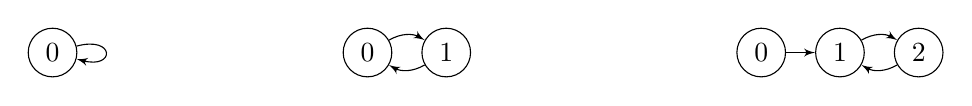
\begin{tikzpicture}
        \tikzset{vertex/.style = {shape=circle,draw,minimum size=1.5em}}
        \tikzset{edge/.style = {->,> = latex'}}
        % vertices
        \node[vertex] (a0) at (0,0) {0};
        \node[vertex] (b0) at (4,0) {0};
        \node[vertex] (b1) at (5,0) {1};
        \node[vertex] (c0) at (9,0) {0};
        \node[vertex] (c1) at (10,0) {1};
        \node[vertex] (c2) at (11,0) {2};
        %edges
        \draw[edge] (a0) to [loop right] ();
        \draw[edge] (b0) to [bend left] (b1);
        \draw[edge] (b1) to [bend left] (b0);
        \draw[edge] (c0) to (c1);
        \draw[edge] (c1) to [bend left] (c2);
        \draw[edge] (c2) to [bend left] (c1);
        
    \end{tikzpicture}

    \caption[Caption for LOF]{Valid number systems\footnotemark\ without any condition
    on \emph{next}}
    \end{figure}
    \footnotetext{It's important to keep in mind what makes one number system different
    from another is how the nodes are linked, it's not about what symbol we keep for each
    node like 0, 1, 2}

    Is this enough? Not really, as we can still think of counterexamples, like
    $next(0) = 1, next(1) = 2, next(2) = 1$. Basically we have ensured that \emph{next}
    doesn't loop back to 0. But we must ensure that it doesn't loop back at all 
    (or even to the same number). How we shall do this is to add the restriction that 
    \emph{next} should not point to a number which has already been mapped to i.e. we make
    it a one-one function. Let's now add these conditions to our axioms:

    \begin{tcolorbox}[colback=blue!10!white, colframe=blue!50!black]
        \begin{enumerate}
            \item $\exists n \ n = 0$
            \item $\forall n \ \exists m \ (m = next(n))$
            \begin{enumerate}
                \item $\forall n \ next(n) \neq 0$
                \item $\forall m \ \forall n \ next(m) = next(n) \implies m = n$
            \end{enumerate}
        \end{enumerate}
    \end{tcolorbox}

    \begin{figure}[ht]
    \centering
    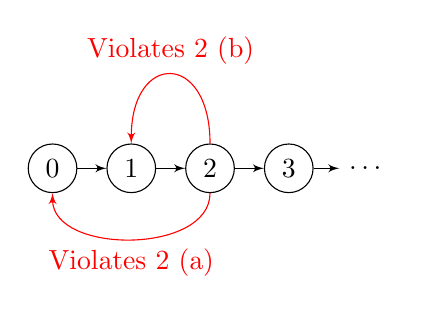
\begin{tikzpicture}
        \tikzset{vertex/.style = {shape=circle,draw,minimum size=1.5em}}
        \tikzset{edge/.style = {->,> = latex'}}
        % vertices
        \node[vertex] (0) at (0,0) {0};
        \node[vertex] (1) at (1,0) {1};
        \node[vertex] (2) at (2,0) {2};
        \node[vertex] (3) at (3,0) {3};
        \node (ellipsis) at (4,0) {\ldots};
        %edges
        \draw[edge] (0) to (1);
        \draw[edge] (1) to (2);
        \draw[edge] (2) to (3);
        \draw[edge] (3) to (ellipsis);
        \draw[red, edge] (2) to [in=90, out=90, looseness=3] node[midway, above] {Violates 2 (b)} (1);
        \draw[red, edge] (2) to [in=270, out=270, looseness=1] node[midway, below] {Violates 2 (a)} (0);
    \end{tikzpicture}
    \caption{Diagrammatic explanation of why \emph{next} always points to a new number}
    \end{figure}

    It turns out our axioms are still not complete. We have ensured that \emph{next}
    always points to a new number, but we haven't really ensured that every natural
    number can be formed by applying \emph{next} to 0 a finite number of times. 
    Here are some counterexamples:
    \begin{enumerate}
        \item $\left\{0, \frac{1}{3}, \frac{2}{3}, \dots\right\}$ where $next(n) = n+1$ 
        \item $[0, \infty)$ where $next(n) = n+1$
    \end{enumerate}
    
    By repeatedly applying \emph{next} to our growing chain, we should end up 
    with the set of all natural numbers. A neat way of stating this is to just
    keep an axiom that induction itself works i.e. if a statement is true for 
    $0, next(0), next(next(0)), \dots$ it must be true for all natural numbers.
    So here is our final set of axioms, which does lead only to our natural numbers:

    \begin{tcolorbox}[colback=blue!10!white, colframe=blue!50!black]
        \begin{enumerate}
            \item $\exists n \ n = 0$
            \item $\forall n \ \exists m \ (m = next(n))$
            \begin{enumerate}
                \item $\forall n \ next(n) \neq 0$
                \item $\forall m \ \forall n \ next(m) = next(n) \implies m = n$
            \end{enumerate}
            \item $[P(0)]  [\forall n \ \{P(n) \implies P(next(n))\}] \implies [\forall n \ P(n)]$
        \end{enumerate}
    \end{tcolorbox}

    \begin{exercise}
        Prove that $\forall n \ next(n) \neq n$. Can we have this statement instead of 
        2 (b) to define natural numbers?
    \end{exercise}
    \begin{solution}
        Proof by induction \\
        Define $P(n)$ to be $\ next(n) \neq n$. $P(0)$ is true from 2 (a). \\
        Also, $next(n) \neq n \implies next(next(n)) \neq next(n)$ as \emph{next} is one-
        one (or contrapositive of 2 (b)). This is basically $P(n) \implies P(next(n))$. \\
        From this we conclude $P(n)$ i.e. $next(n) \neq n$ for all $n$. \\
        This can't be used instead of 2 (b). Counterexample: $next(0) = 1, next(1) = 2, next(2) = 1$.
    \end{solution}

    \begin{exercise}
        Instead of keeping induction as an axiom, we could ensure that there are no other
        starting points for a chain other than 0. This might ensure that all numbers are
        part of the chain starting from 0. 

        Can we replace axiom 3 with the following: \\ 
        $\forall n \ n \neq 0 \iff \exists m \ next(m) = n$
    \end{exercise}
    \begin{solution}
        No, we have a counterexample, take the set \\ 
        $\{0, 1, 2, \dots\} \cup \{\dots, -1.5, -0.5, 0.5, 1.5, \dots\}$ where $next(n)$ is the standard $n+1$. \\
        It satisfies the new set of 3 axioms but aren't equivalent to natural numbers.
    \end{solution}

    \begin{exercise}
        Is there a more concrete way to show that from axiom 3 that all natural numbers
        can be obtained composing $next$ to 0 a finite (including 0) number of times?
    \end{exercise}
    \begin{solution}
        Let $P(n)$ denote $n$ obtained composing \emph(next) to 0 a finite (including 0) 
        number of times. $P(0)$ is obviously true. It's also clear that $P(n) \implies P(next(n))$,
        as if $n$ can be written as $next(next(\dots(next(0))\dots))$, $next(n)$ can also be written
        that way by just composing one more \emph{next} to the expression. 
        This completes our proof.

        Another way we can do this question is proof by contradiction.
        Assume there are some numbers not in the infinite chain starting from 0.
        We define our predicate to be true for values in the infinite chain starting
        from 0, and false for every other value.

        \begin{figure}[ht]
            \centering
            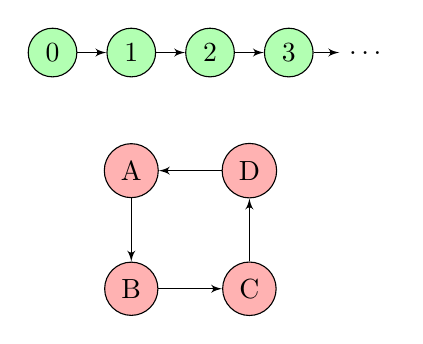
\begin{tikzpicture}
                \tikzset{vertex/.style = {shape=circle,draw,minimum size=1.5em}}
                \tikzset{edge/.style = {->,> = latex'}}
                % vertices
                \node[vertex, fill=green!30] (0) at (0,0) {0};
                \node[vertex, fill=green!30] (1) at (1,0) {1};
                \node[vertex, fill=green!30] (2) at (2,0) {2};
                \node[vertex, fill=green!30] (3) at (3,0) {3};
                \node (ellipsis) at (4,0) {\ldots};

                \node[vertex, fill=red!30] (a) at (1,-1.5) {A};
                \node[vertex, fill=red!30] (b) at (1,-3) {B};
                \node[vertex, fill=red!30] (c) at (2.5,-3) {C};
                \node[vertex, fill=red!30] (d) at (2.5,-1.5) {D};
                %edges
                \draw[edge] (0) to (1);
                \draw[edge] (1) to (2);
                \draw[edge] (2) to (3);
                \draw[edge] (3) to (ellipsis);

                \draw[edge] (a) to (b);
                \draw[edge] (b) to (c);
                \draw[edge] (c) to (d);
                \draw[edge] (d) to (a);
            \end{tikzpicture}
            \caption{Our predicate is true for green cells and false for the red cells}
            \end{figure}
    \end{solution}

    This predicate satisfies $P(0)$ is true. It also satisfies $P(n) \implies P(next(n))$,
    because if $P(n)$ is true only for the green cells, and green cells point to only green cells.
    So induction steps are done, but $P(n) \forall n$ is false. So we have a contradiction.

    \section{Lecture 02}

    To extend our definition, let's define $\leq$ operator.

    \begin{tcolorbox}[colback=blue!10!white, colframe=blue!50!black]
        \begin{enumerate}
            \item $\forall n \ \leq(0, n)$ is true
            \item $\forall n \ \leq(next(n), 0)$ is false
            \item $\forall n \  \forall m \ [\leq(next(n), next(m))\ = \ \leq(n, m)]$
        \end{enumerate}
    \end{tcolorbox}

    \begin{figure}[ht]
    \centering
    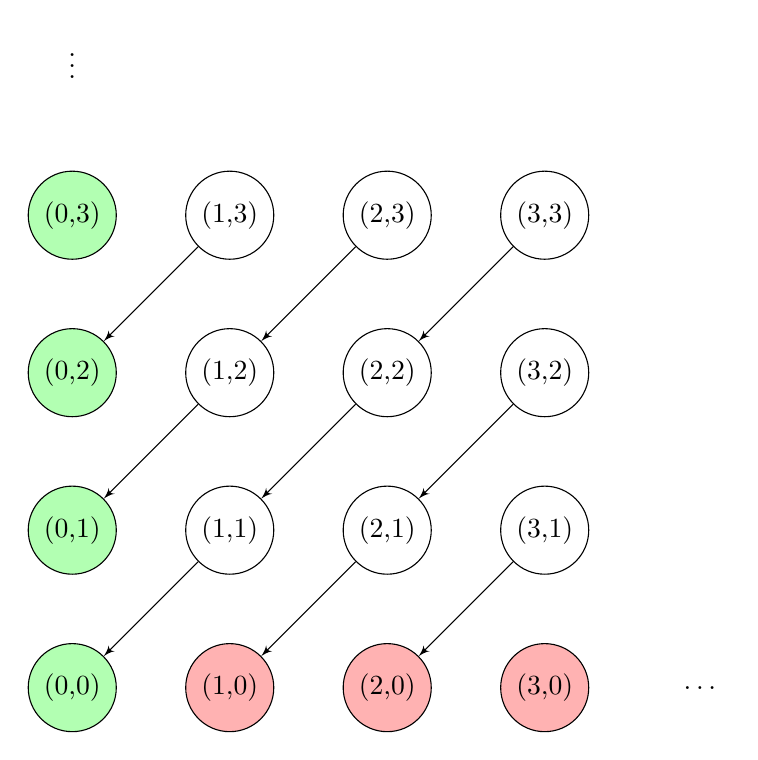
\begin{tikzpicture}
        \tikzset{vertex/.style = {shape=circle,draw,minimum size=1.5em}}
        \tikzset{edge/.style = {->,> = latex'}}

        % vertices
        \foreach \x in {0,...,3}
            \node[vertex, fill=green!30] (0-\x) at (0, 2*\x) {(0,\x)};
        \node (e1) at (0,8) {\vdots};

        \foreach \y in {1,2,3}
            \node[vertex, fill=red!30] (\y-0) at (2*\y,0) {(\y,0)};
        \node (e2) at (8,0) {\ldots};

        \foreach \x in {1,2,3}
            \foreach \y in {1,2,3}
                \node[vertex] (\x-\y) at (2*\x,2*\y) {(\x,\y)};
        

        %edges
        \draw[edge] (1-1) to (0-0);
        \draw[edge] (2-2) to (1-1);
        \draw[edge] (3-3) to (2-2);
        \draw[edge] (2-1) to (1-0);
        \draw[edge] (1-2) to (0-1);
        \draw[edge] (2-3) to (1-2);
        \draw[edge] (3-2) to (2-1);
        \draw[edge] (1-3) to (0-2);
        \draw[edge] (3-1) to (2-0);

    \end{tikzpicture}
    \captionsetup{justification=centering}  % <-- Center the caption
    \caption{Diagrammatic representation of how $\leq$ is defined \\
    $\leq$ is defined as true for green cells, false for red cells \\
    $(A) \rightarrow (B)$ denotes $(A)$ is defined by $(B)$}
    \end{figure}

    From the figure it's intuitive (hopefully) that $\leq(m,n)$ is defined for all $m$ and $n$,
    (3) kind of gives a recursive definition. 
    But how do we prove this? Since our predicate has 2 input variables, there
    is some sort of nested induction.\\
    Take $P(m)$ to be $\forall n \ \leq(m,n)$ is defined. \\
    $P(0)$ is defined from (1).\\
    Now assume $\forall n \ \leq(m,n)$ is defined (which is $P(m)$) \\
    We have to prove $\forall n \ \leq(next(m),n)$ is defined (which is $P(next(m)))$ \\
    The thing is, there's no direct way to proceed from here. It's clear that we somehow
    want to use (3) but we can't as we have $\leq(next(m),n)$ instead of $\leq(next(m),next(n))$.
    How we proceed is we take $Q(n)$ as $\leq(next(m),n)$ is defined, which is want we want to prove
    to complete the induction, and prove $Q(n)$ using induction itself!
    (Note that for the $Q(n)$ statement, $m$ is fixed!)
    $Q(0)$ is true as $\leq (next(m), 0)$ is defined as false. \\
    Now assume $Q(n)$ is true i.e. $\leq(next(m),n)$ is defined. \\
    $Q(next(n))$ is $\leq(next(m),next(n))$ which is $\leq(m,n)$ which is defined, as it is $P(m)$.
    So we proved $\forall n \ Q(n)$, which is the inner induction complete. \\
    This also completes the outer induction.

    \begin{exercise}
        Prove that $\leq(a,b) \ \land \ \leq(b,a) \implies a = b$
    \end{exercise}
    \begin{solution}
        Nested induction on $a$, $b$.\\
        Let $P(a)$ be $\forall b \ \leq(a,b) \ \land \ \leq(b,a) \implies a = b$ \\
        First we need to show that $P(0)$ is true. $\leq(0,b)$ is always true, also
        we can see that $\leq(b,0)$ is true implies $b$ is $0$ as if it's not the case,
        $b$ can be written as $next(k)$ and $\leq(next(k),0)$ is false. \\
        Now for the induction, assume $\leq(a,b) \ \land \ \leq(b,a) \implies a = b$ \quad ($\ast$)\\
        To prove: $\leq(next(a),b) \ \land \ \leq(b,next(a)) \implies next(a) = b$ \\
        Nested induction now, take the above as $P(b)$. 
        \begin{adjustwidth}{2cm}{0cm}
            $P(0)$ is a vacuous truth as $\leq(next(a),0)$ is false. \\
            Now assuming $P(b)$ we have to prove $P(next(b))$, which is \\
            $\leq(next(a),next(b)) \ \land \ \leq(next(b),next(a)) \implies next(a) = next(b)$ \\
            But this is just equivalent to ($\ast$), as LHS of the implication can be 
            simplified by the recursive definition of $\leq$ and RHS of the implication can be 
            simplified with one-oneness of \emph{next}. \\
            So inner induction is complete.
        \end{adjustwidth}
        This also completes outer induction as we have proved $\forall b \ P(b)$
    \end{solution}

    \begin{exercise}
        Prove that $\leq(a,b) \ \land \ \leq(b,c) \implies \leq(a,c)$
    \end{exercise}
    \begin{solution}
        Nested induction again\dots \\
        Let $P(a)$: $\forall b \ \forall c \ \leq(a,b) \ \land \ \leq(b,c) \ \implies \ \leq(a,c)$ \\
        $P(0)$ is true as RHS of implication is always true. \\
        Now assume $P(a)$: $\forall b \ \forall c \ \leq(a,b) \ \land \ \leq(b,c) \ \implies \ \leq(a,c)$ \quad $(\ast)$ \\
        To prove $P(next(a))$: $\forall b \ \forall c \ \leq(next(a),b) \ \land \ \leq(b,c) \ \implies \ \leq(next(a),c)$
        \begin{adjustwidth}{1cm}{0cm}
            Let $Q(b)$: $\forall c \ \leq(next(a),b) \ \land \ \leq(b,c) \ \implies \ \leq(next(a),c)$ \\
            $Q(0)$ is true as first term of LHS of implication is false. \\
            Now assuming $Q(b)$ we have to prove $Q(next(b))$, which is: \\
            $\forall c \ \leq(next(a),next(b)) \ \land \ \leq(next(b),c) \ \implies \ \leq(next(a),c)$
            \begin{adjustwidth}{1cm}{0cm}
                Let $R(c)$: $\leq(next(a),next(b)) \ \land \ \leq(next(b),c) \ \implies \ \leq(next(a),c)$ \\
                $R(0)$ is true as second term of LHS of implication is false. \\
                Now assume $R(c)$, we have to prove $R(next(c))$, which is: \\
                $\leq(next(a),next(b)) \ \land \ \leq(next(b),next(c)) \ \implies \ \leq(next(a),next(c))$ \\
                This can be reduced by the recursive definition to ($\ast$) which is assumed as true.
            \end{adjustwidth} 
        \end{adjustwidth}
        That completes all the induction layers.
    \end{solution}

    \begin{exercise}
        Prove that $\leq(a, next(b)) \ \implies \ [\leq(a,b)] \lor [a=next(b)]$ \\
        Use this to prove $[\leq(a,b)] \land [\leq(b,next(a))] \ \implies \ [b=a] \lor [b=next(a)]$
    \end{exercise}
    \begin{solution}
        Let $P(a)$: $\forall b \ \leq(a, next(b)) \ \implies \ [\leq(a,b)] \lor [a=next(b)]$ \\
        $P(0)$ is true as $\leq(0,b)$ is always true. \\
        Now assuming $P(a)$, we have to prove $P(next(a))$.
        \begin{adjustwidth}{1cm}{0cm}
            Let $Q(b)$: $\leq(next(a), next(b)) \ \implies \ [\leq(next(a),b)] \lor [next(a)=next(b)]$ \\
            $Q(0)$: $\leq(a, 1) \ \implies \ [\leq(a,0)] \lor [a=1]$ \\
            We can first simplify $\leq(a,0)$ to $a=0$ using Exercise 2.1's property. \\
            Let's take $Q(0)$ as $R(a)$ and prove that using induction.
            \newpage
            \begin{adjustwidth}{1cm}{0cm}
                $R(0)$ is true as $\leq(a,0)$ is true. \\
                Now assuming $R(a)$ we have to prove $R(next(a))$. \\
                $\leq(next(a),1) \implies \leq(a,0) \implies a=0 \implies next(a)=1$ so $R(next(a))$ is true \\
                So $R(a)$ is true for all a.
            \end{adjustwidth}
            Now assuming $Q(b)$ we have to prove $Q(next(b))$ \\
            But that can be reduced to just $P(a)$ which is assumed as true. \\
            This completes the induction.
        \end{adjustwidth}
        
        For the second part, we know : \\
        $\leq(b, next(a)) \ \implies \ [\leq(b, a)] \lor [b = next(a)]$ \\
        And if $\leq(b, a)$ since we also know $\leq(a, b)$, $b = a$.

        This exercise shows that there is no number in-between $n$ and $next(n)$ 
    \end{solution}

    We now define the addition function $add(m, n)$: 
    \begin{tcolorbox}[colback=blue!10!white, colframe=blue!50!black]
        \begin{enumerate}
            \item $add(0, m) = m$
            \item $add(next(n), m) = next(add(n, m))$
        \end{enumerate}
    \end{tcolorbox}
    It's not too hard to show this sufficiently defines addition by taking $P(n)$ as
    [$add(n, m)$ is defined] and using induction.

    \begin{exercise}
        Prove that $add(add(a,b), c) = add(a, add(b,c))$ which is the associative property
    \end{exercise}
    \begin{solution}
        We can somehow avoid nested induction for once :) \\
        Let $P(a)$ be $\forall b \ \forall c \ add(add(a,b), c) = add(a, add(b,c))$ \\
        To prove $P(0)$, $LHS = add(add(0,b), c) = add(b,c)$ and $RHS = add(0, add(b,c)) = add(b,c)$ \\
        To prove $P(next(a))$, assuming $P(a)$ is true: \\
        $LHS = add(add(next(a),b), c) = add(next(add(a,b)), c) = next(add(add(a,b), c))$ \\
        $RHS = add(next(a), add(b,c)) = next(add(a, add(b,c)))$ \\
        And from $P(a)$ these both are equal.
    \end{solution}

    \begin{exercise}
        Prove that $add(a,b) = add(b,a)$ which is the commutative property
    \end{exercise}
    \begin{solution}
        Lot of induction again :( \\
        Let $P(a)$ be $\forall b \ add(a,b) = add(b,a)$ \\
        $P(0)$ is $\forall b \ add(0,b) = b = add(b,0)$, this itself has to be done by induction on b. \\
        Now assume $P(a)$ which is $\forall b \ add(a,b) = add(b,a)$ \quad ($\ast$) \\
        Basically whenever we have $a$ in the add function we can swap stuff. \\
        To prove: $P(next(a))$ which is $\forall b \ add(next(a),b) = add(b,next(a))$ \\
        We can simplify LHS a bit: $add(next(a),b) = next(add(a,b)) = next(add(b,a))$ from ($\ast$)
        \begin{adjustwidth}{1cm}{0cm}
            Let $Q(b)$ be $add(b, next(a)) = next(add(b,a))$ \quad ($\ast\ast$) \\
            $Q(0)$ is true as we get $LHS = RHS = next(a)$ \\
            Now assume $Q(b)$, we have to prove $Q(next(b))$ \\
            LHS for this is $add(next(b), next(a)) = next(add(b, next(a)))$ \\
            RHS is $next(add(next(b,a)))$ which is $next(next(add(b,a)))$ \\
            And from ($\ast\ast$) both of these are equal
        \end{adjustwidth}
        This completes all the induction.
    \end{solution}

    \newpage
    \begin{exercise}
        Prove that $\leq(a,b) \ \implies \ \exists c$ such that $add(a,c) = b$
    \end{exercise}
    \begin{solution}
        Let $P(a)$ be the above statement for all $b$. \\
        $P(0)$ is true as $c = b$ works. \\ 
        Now assume $P(a)$ is true. \quad ($\ast$) \\
        We have to prove $P(next(a))$, take this as $Q(b)$.
        \begin{adjustwidth}{1cm}{0cm}
            $Q(0)$ is vacuously true as $\leq(next(a), 0)$ is false. \\
            Now assuming $Q(b)$ we have to prove $Q(next(b))$ \\
            $\leq(next(a), next(b)) \ \implies \ \leq(a,b)$ \\
            So from ($\ast$) we know $\exists c$ such that $add(a,c) = b$ \\
            But this also implies $add(next(a), c) = next(b)$ \\
            This proves $Q(next(b))$ which completes all the induction.
        \end{adjustwidth}
        This exerise in a way defines subtraction, $c = b-a$
    \end{solution}

    \section{Lecture 03}
    Rather than using induction, there's an equivalent way to define natural numbers called
    well-ordering principle. Here are the axioms:

    \begin{tcolorbox}[colback=blue!10!white, colframe=blue!50!black]
        \begin{enumerate}
            \item $\exists n \ n = 0$
            \item $\forall n \ \exists m \ (m = next(n))$
            \begin{enumerate}
                \item $\forall n \ next(n) \neq 0$
                \item $\forall m \ \forall n \ next(m) = next(n) \implies m = n$
                \item $\forall n \ [n = 0] \lor [\exists m \ n = next(m)]$
            \end{enumerate}
            \item $\exists \ \leq$
            \begin{enumerate}
                \item $\forall n \ \lnot \leq(next(n), n)$
                \item $\forall P \ [(\exists n \ P(n)) \ \implies \ \exists n \ (P(n) \ \land \ \forall m(P(m) \implies n \leq m))]$
            \end{enumerate}
        \end{enumerate}
    \end{tcolorbox}

    This might look like it's very complicated using predicate logic, so let's try to see
    what all this means. So the beginning is pretty much like the previous axioms, but 2(c)
    is new. It basically says every number is either 0 or is the \emph{next} of some other number.
    We'll later see how this axiom helps in proving induction itself.

    What does the third axiom say? It says there exists \textbf{some} predicate $\leq$, which 
    is not necessarily the $\leq$ we saw in Lecture 02. But anyways there's some predicate
    $\leq$ which `orders' the natural numbers. What exactly do we mean by that? 3(a) says
    \emph{next} of any number is greater than it. 3(b) says that for all predicates $P$, if
    there is at least one number for which $P$ is true, there will a `smallest' number for
    which it is true. How we write this formally is that there is some $n$ for which $P(n)$ is
    true and for every other $m$ for which it is true, $n \leq m$.

    Let's see how induction is true from these axioms. We prove induction by contradiction.
    Assume there is a predicate $P$ such that $P(0)$ is true, and $P(n) \implies P(next(n))$.
    But $\forall n \ P(n)$ is false, that is there's some $n$ for which $\lnot P(n)$ is true.
    Let the smallest $n$ that satisfies this be $n_0$ (we're using 3(b) here).
    $n_0 \neq 0$ as $P(0)$ is true. So from 2(c) there's $m$ such that $next(m) = n_0$.
    Is $P(m)$ true? If it was, $P(m) \implies P(next(m))$, which would make $P(n_0)$ true.

    So $P(m)$ is false, but haven't we just found a number smaller than $n_0$ which satisfies
    $\lnot P(n)$, which contradicts well-ordering? From 3(a) we know $\leq(n, m)$ is false\footnote
    {Without 3(a) we can't actually conclude this, remember this isn't our familiar
    $\leq$, this is just an arbitrary predicate which satisfies well-ordering}.
    So from 3(b) we can get our contradiction, but remember the predicate we are using is 
    $\lnot P$ instead of $P$. We have $n$ such that $\lnot P(n)$, so 3(b) guarantees
    there exists $n_0$ such that $\lnot P(n)$ is true, and for all other $m$ that
    satisfies $\lnot P(n)$, $\leq(n,m)$. So 3(a) and 3(b) form our contradiction.

    \begin{exercise}
        We have seen how 2(c) was used in proving induction, but maybe even without it
        maybe we get only natural numbers? Is there a number system which isn't natural numbers
        but satisfies everything except 2(c)?
    \end{exercise}

    \begin{solution}
        In fact there are.
        $\{0, 1, 2, \dots, \omega, \omega+1, \omega+2, \dots\}$ form a number system. \\
        Here $\leq$ is what you'd expect it to be, the numbers are arranged in order 
        already, and $\omega$ is greater than all the natural numbers. 
        $\leq$ satisfies all the properties it needs to, even things like 
        the transitive property. But 2(c) forbids such things are there is no $n$
        such that $next(n) = \omega$. These are actually called the ordinal numbers.
        Thing is, we get many useful number systems if we make small changes to our axioms,
        for example if we remove $next(n) \neq 0$ we get modular arithmetic.

        \begin{figure}[ht]
            \centering
            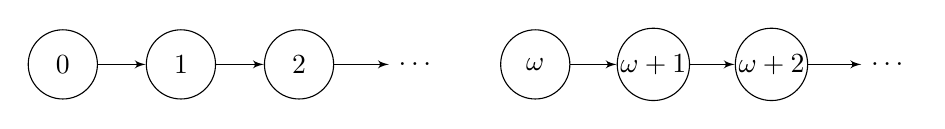
\begin{tikzpicture}
                \tikzset{vertex/.style = {shape=circle,draw,minimum size=2.5em}}
                \tikzset{edge/.style = {->,> = latex'}}
                % vertices
                \node[vertex] (0) at (0,0) {0};
                \node[vertex] (1) at (1.5,0) {1};
                \node[vertex] (2) at (3,0) {2};
                \node (e1) at (4.5,0) {\ldots};
                \node[vertex, inner sep=0.5pt] (w) at (6,0) {$\omega$};
                \node[vertex, inner sep=0.5pt] (w1) at (7.5,0) {$\omega + 1$};
                \node[vertex, inner sep=0.5pt] (w2) at (9,0) {$\omega + 2$};
                \node (e2) at (10.5,0) {\ldots};

                %edges
                \draw[edge] (0) to (1);
                \draw[edge] (1) to (2);
                \draw[edge] (2) to (e1);
                \draw[edge] (w) to (w1);
                \draw[edge] (w1) to (w2);
                \draw[edge] (w2) to (e2);
            \end{tikzpicture}
            \caption{Valid number system without 2(c)}
        \end{figure}        

    \end{solution}

    \section{Lecture 04}

    The last lecture we saw the well-ordering principle, and showed how induction
    follows from it. Once that's true, we have basically confirmed that it also
    defines the natural numbers. Now let's try to prove the well-ordering principle
    from the induction axioms. 

    Proving 2(c) is not too hard using induction, actually the proof sounds silly.
    $P(0)$ is true as $0 = 0$\footnote{Where's my fields medal for observing this}.
    And to prove $P(next(n))$ we need to find $m$ such that $next(m) = next(n)$ and
    $m = n$ works for this.

    Now for 3(a). Remember that for axiom 3, we just need to find one predicate $\leq$
    which works, and we claim that the $\leq$ we defined in Lecture 02 works. 3(a) is
    also done by induction, take $P(n)$ to be $\leq(next(n),n)$ is false. $P(0)$ is 
    true as $\leq(next(n), 0)$ is always false. $P(n) \implies P(next(n))$ is also clear as
    $\leq(next(next(n)), next(n)) \ = \ \leq(next(n), n)$.

    3(b) is done by contradiction. So suppose there's a predicate $P$ such that $P(n)$
    is true for some $n$, but there's no smallest $n$ for which $P(n)$ is true. How our
    contradiction will go is by showing $P(n)$ is false for all $n$. We will do this by 
    showing if $P(0)$ is false, $P(1)$ is false, \dots, $P(n)$ is false, this implies
    $P(next(n))$ is false\footnote{This is something called strong induction; for proving
    something for $next(n)$, instead of just assuming it for $n$, we assume it true for
    $0$ to $n$. This is equivalent to induction actually}.

    We take $Q(n): \forall m \ (m \leq n) \implies (\lnot P(m))$ or in other words,
    $Q(n)$ says $P(k)$ is false for $0 \leq k \leq n$. What is $Q(0)$? $m \leq 0
    \implies P(m)$ is false or simply, $P(0)$ is false. This is right as if $P(0)$
    were true, 0 is clearly a smallest $n$ for which $P(n)$ is true.

    \newpage
    Now let's try to induct on $Q(n)$. Is it possible that $Q(n)$ is true and 
    $Q(next(n))$ is false? This would mean there exists $m \leq next(n)$ such that 
    $P(m)$ is true, at the same time $m \nleq n$, which means $m = next(n)$ (See exercise 2.3). 
    But this $m$ we found would then be a smallest $k$ for which $P(k)$ is true. Why? 
    Let $k$ be such that $P(k)$ is true, we know $k \nleq n$ from $Q(n)$.
    So we have to show
    if $k \nleq n$, $m = next(n) \leq k$. This is equivalent to showing that 
    $[k \leq n] \lor [next(n) \leq k]$ which can be shown by nested induction. So we got
    that it's impossible, $Q(n)$ has to imply $Q(next(n))$. This would then mean
    $Q(n)$ is true for all $n$ which is the same thing as $P(n)$ is false for all $n$
    \footnote{As $Q(n)$ implies $\lnot P(n)$},
    which is a contradiction.

    This proof does use a lot of English, but it's still correct and can be written in predicate
    logic, but that takes away the intuition.

    \begin{exercise}
        Prove that $[a \leq b] \lor [next(b) \leq a]$. Is it possible for both of these to be true?
    \end{exercise}

    \begin{solution}
        Let $P(a)$ be $\forall b \ [a \leq b] \lor [next(b) \leq a]$. \\
        $P(0)$ is true as $0 \leq b$. Now assume $P(a)$. \\
        $P(next(a))$ is $\forall b \ [next(a) \leq b] \lor [b \leq a]$.
        \begin{adjustwidth}{1cm}{0cm}
            Let $Q(b)$ be $[next(a) \leq b] \lor [b \leq a]$. \\
            $Q(0)$ is true as $0 \leq a$. \\
            $Q(next(b))$ is equivalent to $P(a)$ which is assumed to be true.
        \end{adjustwidth}
        This completes the induction.

        No it's not possible for both to be true. \\
        $a \leq b$ and $b \leq next(b)$ implies $a \leq next(b)$. \\
        This along with $next(b) \leq a$ means $a = next(b)$. \\
        But $a = next(b) \leq b$ is clearly false, so we get a contradiction.
    \end{solution}

    \section{Lecture 05}
    We discuss some common mistakes made while doing induction proofs. Say you want
    to prove something for all objects which can have sizes 0, 1, 2, \dots.
    In the induction step, we can assume the property is true for all objects of size $n$.
    We must then show it's true for \emph{all} objects of size $n+1$, not just \emph{some}
    objects. Take the following example: \\
    Every sequence of $n$ numbers with sum $2n-1$ must contain an occurence of $1$ \\
    $\forall n \ \forall S \ [L(s) = n] \land [sum(s) = 2n-1] \implies occurs(S,1)$ \\
    This statement is clearly wrong, take the counterexample sequence $\{0, 3\}$. But
    here's a proof using induction which has a mistake. First let's define a sequence
    and define how induction works to prove something for all sequences. \\
    Definition of sequence:
    \begin{enumerate}
        \item $\lambda$ is a sequence which is an empty sequence
        \item If $S$ is a sequence, $insert(S,n)$ is a sequence for all numbers $n$
    \end{enumerate}
    Induction for sequences:
    \begin{enumerate}
        \item $P(\lambda)$ is true
        \item $\forall S \ [P(S)] \implies [\forall n \ P(insert(S, n))]$ 
    \end{enumerate}

    Clearly, these aren't complete definitions, lot of details are assumed to be understood.
    But with enough conditions added, they will define sequences without any ambiguities. 
    
    So for our wrong proof we just do induction on $n$, not actually sequence induction.
    $P(0)$ is vacuously true as sum of sequence of length 0 is just 0. Now we do induction.
    Assume $P(n)$ is true. Now a sequence of length $n+1$ can be formed by $insert(S, 2)$
    where $S$ is a sequence of length $n$. Assuming our new sequence has sum $2(n+1)-1$, 
    $S$ will have sum $2(n+1)-1 - 2 = 2n-1$, so by induction 1 is in $S$, which means
    1 is in our sequence of length $n+1$.

    Why is this proof wrong? We haven't proved our statement for \emph{all} sequences of length
    $n+1$, just for the sequences with ending element 2. We have only proved that there exists
    some sequence which has a 1, not all sequences have a 1.

    So let's modify our statement to be true and then prove it properly by induction. Let's
    add the restriction that our sequence contains only \emph{non-zero} numbers. Now
    our statement is true, because if it didn't contain a 1, the sum would be at least
    $2 + 2 + \dots + 2 = 2n$. So we should be able to prove this by induction.
    
    For $n = 0$ again the statement is vacuously true. For $n = 1$ it must be true as 
    well because the only sequence with sum $2\times1-1$ is $\{1\}$. So let's assume 
    it's true for sequences of length $n$. Every sequence of length $n+1$ is formed by 
    inserting a number $x$ to a sequence of length $n$, let's go case by case.

    $x \neq 0$ from our conditions. If $x = 1$ we are done, our sequence has a 1. If
    $x = 2$, the rest of the sequence with length $n$ has sum $2n-1$ so it has a 1 by
    induction, so far so good. But what if $x > 2$? Intuitively it's still true that 
    the rest of the sequence should contain a 1 right, because the sum should be smaller 
    than $2n-1$, but we can't exactly proceed by induction as our statement says nothing 
    about such sequences. So to prove our statement, we actually make a stronger claim:

    Every non-empty sequence $S$ of length $n$ with $sum(S) \leq 2n-1$ contains a $1$
    
    If we prove this statement by induction, we also solve the question as this is a 
    stronger statement i.e. it is claiming something about a larger set of sequences. 
    So let's just modify our proof to prove this statement. Again $P(0)$ is vacuously true.

    $x \neq 0$ from our conditions. If $x = 1$ we are done, our sequence has a 1.
    If $x \geq 2$, the sum of the rest of the sequence is $\leq 2(n+1)+1-x \leq 2n-1$.
    So the rest of the sequence must contain a 1 by our induction assumption, this completes
    the induction.

    The take away message is that in order to prove a statement by induction, sometimes 
    we have to make a stronger statement which is easier to prove by induction.

    \textbf{Homework: }Consider a set of $n+1$ positive numbers each of which is atmost
    $2n$. Prove that there exist 2 numbers such that one divides the other.

    \newpage
    \section{Lecture 06}

    We solve the homework question using well-ordering principle and proof by contradiction.
    It turns out that this method is more useful than direct induction for solving decently
    challenging questions, but is equivalent to induction. We assume $n$ is the smallest
    number for which $P(n)$ is false (where $P(n)$ is what we want to prove), 
    and use the fact that $P(k)$ is true for all $k < n$
    to get some sort of contradiction showing that $P(n)$ is in fact true. Remember it's
    important to show a base case, here $n = 1$. In this case the only sets are \{1, 1\}, 
    \{1, 2\} and \{2, 2\} so our statement is true.

    So let $n$ the smallest number for which $P(n)$ is false. Let the sequence for which 
    it is false be $\{a_{1}, a_{2}, \dots, a_{n}, a_{n+1}\}$ and also assume the numbers are
    in ascending order. What can we say about this sequence? Obviously none of the numbers
    are the same, if so they divide each other. Also look at the subsequence of this,
    $\{a_{1}, a_{2}, \dots, a_{n}\}$. If all of the numbers were atmost $2n-2$, the conditions
    for $P(n-1)$ would be satisfied, which would mean two numbers divide each other. And
    if this is true for our subsequence, it's also true for the whole sequence, so we have a contradiction.

    $a_{n}$ must be greater than $2n-2$, and since all terms of are sequence are atmost
    $2n$ and distinct, $a_{n} = 2n-1, a_{n+1} = 2n$. But we can actually still get a
    contradiction, if we consider the subsequence $\{a_{1}, a_{2}, \dots, a_{n-1}, n\}$
    \footnote{Here $n$ is not necessarily the greatest element, the elements aren't in 
    order}.
    Here all terms are atmost $2n-2$ as $a_{n-1} < a_{n} = 2n-1$ and $n \leq 2n-2$. So
    we can apply $P(n-1)$, $x$ and $y$ exist in the sequence such that $x | y$. Is it possible
    that neither of $x$, $y$ are $n$? No, because then we would have 2 numbers in our
    original sequence which divide each other. So $n$ is one of $x,y$. We can also say
    $y = n$, because $x$ can't be $n$, there's no term in the sequence big enough for $n$
    to divide (except $n$ itself). So some $x$ divides $n$. We're not done though, as $n$
    is not part of our original sequence, but $a_{n+1} = 2n$ is! And if $x$ divides $n$, 
    $x$ divides $2n$. So we still have 2 numbers in our original sequence which divide
    each other, so we have a contradiction.

    Let's move to an even more challenging example.

    \textbf{Erd\"{o}s-Ginzburg-Ziv Theorem: }Any sequence of $2n-1$ numbers contains a 
    subsequence of $n$ elements, with their sum being a multiple of $n$. 

    Let $n$ be the smallest number for which the statement is not true. Assume $n$ is 
    composite and $n = pq$ where $p,q > 1$. We show by contradiction that if the statement
    is true for $p, q$ it is true for $n$ (we take care of the case where $n$ is prime later).

    We have $2pq-1$ numbers. Choose $2p-1$ numbers from these. Now from our assumption,
    we can choose $p$ numbers out of these with sum divisible by $p$. Take these numbers
    away and put them in a group $G_{1}$. And for the rest of the $p-1$ numbers, put them
    back into our original sequence, to recycle them. Now again choose $2p-1$ numbers from
    our original sequence, find $p$ of them with sum divisible by $p$, put them away in a 
    group $G_{2}$, and recycle the $p-1$ numbers not chosen. How many groups can we form if 
    we keep doing this? $2pq-1 = (2q-2)p + (2p-1)$, so after finding $2q-2$ groups, we have
    $2p-1$ numbers left. We form a final group of size $p$, and throw away the $p-1$ numbers.

    Now have groups $G_{1}, G_{2}, \dots, G_{2q-1}$ each with sum $k_{1}p, k_{2}p, 
    \dots, k_{2q-1}p$. Now what we do is find $q$ numbers from $k_{1}, k_{2}, \dots,
    k_{2q-1}$ with sum divisible by $q$, say the chosen numbers are $k'_{1}, k'_{2},
    \dots, k'_{q}$. Now think about choosing the numbers from these corresponding groups\dots
    We have $q$ groups of $p$ numbers each, so we have chosen $pq$ numbers. And their
    sum is \\
    $(k'_{1} + k'_{2} + \dots + k'_{q})p = (kq)p$, so the sum is divisible by
    $pq$, thus we found our contradiction. 

    Let's now deal with the case when $n$ is prime. Firstly, let's reduce all numbers
    and our calculations $\mod n$, because we only care about the remainders when
    divided by $n$. Can $\geq n$ numbers from the $2n-1$ be equal? In that case we're
    already done, $n$ numbers from those obviously have a sum divisible by $n$. So let's
    assume each number appears less than $n$ times.
    
    We divide the numbers into $n$ groups: 
    \begin{align*}
        (a_1, &b_1) \\
        (a_2, &b_2) \\
        &\vdots \\
        (a_{n-1}, &b_{n-1}) \\
        (c &)
    \end{align*}

    We also add the restiction that no 2 numbers of each group are equal $\mod n$. Can
    we always do this? Just sort the numbers in ascending order, and put them in the 
    groups in the order $a_1, a_2, \dots, a_{n-1}, c, b_1, b_2, \dots, b_{n-1}$. The only
    way you can have a repetition is if when you add many copies of a number, it somehow
    occupies every spot from $a_i$ to $b_i$. But this would mean the number is present in
    our sequence at least $n+1$ times, which we already concluded is not the case.

    We claim that there's a way to pick 1 number from each group such that the sum is 
    divisible by $n$. How we show this, is by showing that there are at least $n$ 
    different sums we can make by choosing different numbers from each group. Assume we 
    are working just with the first group. We have 2 different sums, $a_1$ and $b_1$.
    If we include the second group, we have 4 sums: $a_1+a_2, a_1+ b_2, b_1+a_2, b_1+b_2$.
    But these sums may not be distinct $\mod n$. So how do we proceed? We induct on the 
    number of groups we are working with; we claim with $i$ groups there are at least $i+1$
    sums we can form. (Here $i$ ranges from $1$ to $n-1$, the $n^{th}$ group has no choice.)

    When $i=1$ it's obvious we have 2 distinct sums, $a_1$ and $b_1$ as $a_1 \neq b_1 \mod n$.
    Now assume the statement is true for $i$, we have to show it's true for $i+1$.
    Let the $i+1$ sums we got from the first set of $i$ groups be $\{s_1, s_2, \dots, s_{i+1}\}$.
    Now by taking the $(i+1)^{th}$ group we get the sums: \\
    $\{s_1+a_{i+1}, s_2+a_{i+1}, \dots, s_{i+1} + a_{i+1}\}$ \\
    $\{s_1+b_{i+1}, s_2+b_{i+1}, \dots, s_{i+1} + b_{i+1}\}$ \\
    It's clear that all elements inside one of these sets are distinct as all the $s$'s are distinct.
    But how do we know 2 elements from different sets are distinct? Note that if there's
    just a single difference between both the sets, we will get $i+2$ new sums, and our induction
    is done. So how do we show each set isn't identical to each other $\mod n$?

    The trick is to show that the sum of numbers in each set aren't equal. If so, the
    difference of the sums would be $0 \mod n$. Note that the difference is just
    $(i+1)(b_{i+1}-a_{i+1})$ as all the $s$ terms cancel. If this was $0 \mod n$, 
    as $n$ is prime, either $i+1$ or $b_{i+1}-a_{i+1}$ is divisible by $n$. But this isn't
    possible as $i+1$ is smaller than $n$
    \footnote{Strictly speaking $i$ ranges from $1$ to $n-1$, so why can't $i+1 = n$?
    But our final induction is from $i = n-2$ to $i+1 = n-1$ so we don't have to deal 
    with this case}
    and by our construction of the groups, $a_{i+1} \neq b_{i+1} \mod n$. So it's 
    impossible for both sets to be same, our induction step is true. 

    Now that our induction is complete, by choosing different elements we can get
    $n$ different sums $\mod n$, so basically we can get any sum $\mod n$, including
    $0 \mod n$ which is what we want. This completes the proof for the whole theorem.

    \section{Lecture 07}

    We move to a new number system, numbers modulo $m$ where $m$ is a fixed number 
    greater than $0$. The axioms for this system are very similar to natural numbers,
    except that $m = 0$ i.e $next(m-1) = 0$. The only axiom which is different from
    natural numbers here is we remove the restriction $next(n) \neq 0$. 

    \begin{figure}[ht]
        \centering
        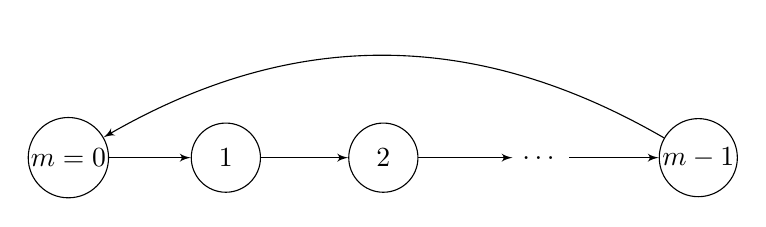
\begin{tikzpicture}
            \tikzset{vertex/.style = {shape=circle,draw,minimum size=2.5em}}
            \tikzset{edge/.style = {->,> = latex'}}
            % vertices
            \node[vertex, inner sep = 0.5pt] (0) at (0,0) {$m = 0$};
            \node[vertex] (1) at (2,0) {1};
            \node[vertex] (2) at (4,0) {2};
            \node (ellipsis) at (6,0) {\ldots};
            \node[vertex, inner sep = 0.5pt] (m-1) at (8,0) {$m-1$};
            %edges
            \draw[edge] (0) to (1);
            \draw[edge] (1) to (2);
            \draw[edge] (2) to (ellipsis);
            \draw[edge] (ellipsis) to (m-1);
            \draw[edge] (m-1) to [bend right] (0);
        \end{tikzpicture}
        \caption{Modulo $m$ number system}
    \end{figure}

        We can rigorously define the function to convert from naturals to numbers 
        modulo $m$, $n \mod m$ is the smallest number $r$ such that $n = qm + r$
        for some $q$. It's clear that $0 \leq r < m$ as if $r \geq m$, there exists $r'$ 
        such that $r = m + r'$ (proof is similar to Exercise 2.6). Substituting this, 
        we get $n = qm + m + r' = (q+1)m + r'$, so we found $r' < r$ which satisfies 
        the condition.

        This is also a well defined notation, as the set $\{ x | n = qm + x\}$ is non-
        empty. $n$ itself is in this set for $q = 0$. And any set which is non-empty 
        will have a least element, which is another way to look at the well-ordering 
        principle (Here $P(x)$ just means $x$ belongs to our set).

        Almost all operations can be defined for numbers $\mod m$. $n \mod m \ + \ k \mod m$
        is defined as $ = (n+k) \mod m$. It's also easy to show that this is commutative
        and associative by swapping around terms in the RHS. 
        Unlike the natural numbers, each number also has
        an additive inverse. This is due to the fact that if you keep adding 1 to a number,
        it will eventually loop to 0.

        How do we define an additive inverse? We must first define an additive identity,
        this is a number $a$ such that $a + n = n \ \forall n$. Clearly $a = 0$ is the 
        additive identity. The additive inverse of $n$ is a number $n'$ such that
        $n + n' = a$. The same can be defined for multiplication, and $1$ is the multiplicative identity.

        In order to talk about mutliplicative inverse, we must first define the greatest
        common divisor (gcd) of 2 numbers. For two positive numbers $a$, $b$, consider the 
        sets: \\
        $X = \{ r > 0 \mid \exists x,y \ xa = yb + r \}$ \\
        $Y = \{ r > 0 \mid \exists x,y \ xb = ya + r \}$ \\
        Both these sets aren't empty, for $x = 1$ and $y = 0$, $a, b$ belong to $X,Y$
        respectively. So each set has a well defined smallest element. The gcd of $a,b$
        is defined as the smallest element in $X \cup Y$.
        
        Another way to think about this is $X \cup Y$ is that it contains the difference
        of any multiple of $a$ with any multiple of $b$, or even can be taken as the set
        of all integer linear combinations of $a, b$ (which are positive). It's not clear that this is the 
        same as the gcd we are used to, but the properties of gcd can be proven from this 
        definition.

        What properties would we like to prove? Firstly we should check that $a \mod g = 0$
        and $b \mod g = 0$. $g$ should also be a multiple of any common divisor of $a, b$ i.e.
        if $d \mid a$ and $d \mid b$ then $d \mid g$.

        \newpage
        Let $g$ be the smallest number in $X \cup Y$. Let's take the case where $g \in X$.
        So there exists $x, y$ such that $xa = yb + g \ (1)$. Now to prove $a \mod g = 0$, let's
        assume by contradiction $a \mod g = g' \neq 0$. This can be written as $a = qg + g' \ (2)$
        from the definition of $mod$. Multiplying (1) by $q$ and adding $g'$ to both sides, we get: \\
        $qxa + g'= qyb + qg + g' = qyb + a$ (from (2)) \\
        Rearranging, $(qy)b = (qx-1)a + g'$ \\ 
        But this would mean $g' \in Y$, contradicting the fact that $g$ is the smallest element 
        in $X \cup Y$.

        The proof is identical for the other case when $g \in Y$, we get $g' \in X$
        which also leads to a contradiction. We conlcude $a \mod g = 0$. Since the 
        definition of gcd is symmetric about $a$ and $b$, we can prove using the same
        method $b \mod g$ = 0.

        Now to prove that every common divisor of $a, b$ divides $g$ too. Let $d$ be 
        such that $a \mod d = 0, b \mod d = 0$. Let $x,y$ be such that $xa = yb + g$
        \footnote{If $g \in Y$ the proof is same}. \\
        $xa \mod d = 0$ \\
        $(yb + g) \mod d = 0$ \\
        $yb \mod d + g \mod d = 0$ \\
        Since, $b \mod d = 0$, $yb \mod d = 0$, so $g \mod d = 0$ (we are done).

        \begin{exercise}
            Prove that if $a \mid bc$ and $gcd(a, b) = 1$, $a \mid c$.
        \end{exercise}
        \begin{solution}
            If $gcd(a, b) = 1$, we have integers $x,y$ such that $ax + by = 1$. Multiplying
            by $c$, $acx + bcy = c$. Since $a \mid acx$, $a \mid bcy$, $ a \mid c$. 
        \end{solution}

        \begin{exercise}
            Prove that if $p$ is prime and $p \mid ab$ then $p \mid a $ or $p \mid b$
        \end{exercise}
        \begin{solution}
            Firstly what's the definition of a prime? $p$ is prime if the only divisors
            of $p$ are 1 and $p$. The statement we want to prove is equivalent to proving
            $p \mid ab$ and $p \nmid a$ means $p \mid b$. We first show that $gcd(p,a) = 1$.
            This is fine, as if $g \mid p$, $g$ is 1 or $p$, and since $g \nmid a$, $g$ is not
            $p$, so $g$ is 1. From here the question is equivalent to the previous exercise.
        \end{solution}

        \begin{exercise}
            Are $X, Y$ in the gcd definition always the same set?
        \end{exercise}
        \begin{solution}
            Yes, they are. In fact both sets contain the gcd and all multiples of it.
            Let's prove that $X = \{ g, 2g, 3g, \dots \}$. The proof is identical for $Y$.
            Let $a' = a/g$, $b' = b/g$. Is it clear that $gcd(a',b') = 1$? Well if it wasn't
            and was equal to say $g'$, $g'$ would divide $a', b'$, and $gg'$ would divide $a, b$
            and this is a contradiction.
            
            Now if we prove we can find $x,y$ such that $xa' = yb' + 1$, we're done, as we can multiply
            both sides by $g$. We're also done if we can find $x$ such that $xa' = 1 \mod b'$.
            Here's how we show that, take the set \\
            $\{ 0, a', 2a', \dots, (b'-1)a' \}$ with $b'$ elements. We claim each element here
            is distinct mod $b'$. If 2 of them have the same remainder, say $ia'$ and $ja'$, 
            this would mean $b' \mid (i-j)a'$. But since $gcd(a',b') = 1$, $b' \mid i-j$. But 
            this is impossible as $i-j < b'$. But now that we have $b'$ distinct elements, we know
            that we can have only maximum $b'$ distinct remainders right, which means that our set
            has all the elements $\mod b'$, including the remainder 1. So we're done, there
            exists $x$ such that $xa' = 1 \mod b'$ which is the same as saying $xa' = yb' + 1$
            (for some $y$).

            Now that we've shown $g \in X$, it's clear that all multiples of $g$ are in $X$,
            as if $xa = yb + g$, $mxa = myb + mg$. All that's left to show is that the \emph{only}
            numbers in $X$ are multiples of $g$. This is also easy as if $xa = yb + r$, and 
            $g \mid xa$, $g \mid yb$, so $g \mid r$.
        \end{solution}

        \newpage
        \begin{exercise}
            Prove the fundamental theorem of arithmetic, that is every number $n$ can 
            be written uniquely as $n = p_1p_2 \dots p_k$ where the primes are written 
            in ascending order.
        \end{exercise}
        \begin{solution}
            First we prove that such a representation exists. We can do this by strong 
            induction. For $n=1$ the statement is trivial, $n=1$ is the representation.
            Now assume the statement is true for all numbers smaller than $n$. If $n$ is
            prime, $n = n$ is our representation. If $n$ is not prime, we can write 
            $n = xy$ for some $x,y > 1$. By induction assumption $x,y$ can be written as
            a product of primes, from there $n$ can be written as a product of primes.

            Now for uniqueness. Again for $n=1$ it is clear, there's no other way to write
            it. Now we'll use well ordering and proof by contradiction. Let $n$ be the 
            smallest number for which there are 2 distinct way to prime factorize it.
            Say $n = p_1p_2 \dots p_n = q_1q_2 \dots q_m$. None of $p_i, q_j$ for all $i, j$
            can be equal as if they were, we could just cancel those terms and get a smaller
            number with 2 different prime factorizations. Now WLOG assume $p_n$ is the largest
            prime in both representations. $p_n \mid q_1q_2 \dots q_m$, $p_n \nmid q_1$ as
            $p_n > q_1$, so $p_n \mid q_2 \dots q_m$. Similarly since $p_n \nmid q_2$, 
            $p_n \mid q_3 \dots q_m$. We can continue doing this and get that $p_n \mid q_m$
            which is a contradiction.
        \end{solution}

    \section{Lecture 08}

    We're going to do some questions regarding divisibility and binomial coefficients.
    To prove that $n$ is divisible by $d$, you can think of a situation where's there
    a collection of $n$ objects. If we can divide this collection into groups such that 
    each group has $d$ elements, we are done. Another way to prove is to divide the 
    collection into $d$ groups such that each group has the same number of elements.

    When we're dealing with binomial coefficients like $\binom{n}{k}$, we can think of
    this as the number of collections of $k$ objects out of $n$ objects in total.

    \begin{exercise}
        If $gcd(n,k) = 1$, prove that $n \mid \binom{n}{k}$
    \end{exercise}
    \begin{solution}
        It's possible to prove this directly. \\
        $k \binom{n}{k} = n \binom{n-1}{k-1}$. So $n$ divides $k \binom{n}{k}$ and
        since $gcd(n,k)=1$, $n$ divides $\binom{n}{k}$. But let's prove this combinatorially.

        We can think of $\binom{n}{k}$ as the number of collections with $k$ objects
        from the set $\{0, 1, \dots, n-1\}$. Suppose we have a collection $\{a_1,
        a_2, \dots a_k \}$. We claim that we can extend this to a group of $n$ collections from this 
        collection. How we do this is by adding $0, 1, 2, \dots, n-1$ to each element, 
        and taking $\mod n$. So the first collection is formed by adding $0$ to each element,
        so it's our original collection itself. For the second collection you add 1 to 
        each element, and so on.

        It's not possible that 2 groups have one common element. Suppose collection $C$ is formed
        from adding $i$ from a collection $C_1$ and $j$ from a collection $C_2$. $C_1$ and $C_2$
        have to be a part of the same group as you get one from adding $i-j$ to the other.

        How do we know these $n$ collections are distinct? Assume 2 of them are same, say the ones where
        you add $i$ and $j$ to the original collection. The difference of their sums $\mod n$ must 
        be 0, and this difference is $k(i-j)$. Since $n \mid k(i-j)$ and $gcd(n,k)=1$, $n \mid (i-j)$.
        This isn't possible as $(i-j) < n$. So now that we can bunch up all collections into groups
        of size $n$, we conclude $\binom{n}{k}$ is divisible by $n$.

        Another solution could be to divide the collections based on their sum $\mod n$. There are
        clearly $n$ groups. And for any collection in a group, you can find a corresponding collection
        in any other group by adding a suitable $i$ to each element. The proof for this is very similar. Once this is 
        shown, we basically have shown each group is of equal size. So $\binom{n}{k}$ is divisible by $n$.
    \end{solution}

    \begin{exercise}
        Is the converse of the above statement true? If $n \mid \binom{n}{k}$ can we say that
        $gcd(n,k)=1$?
    \end{exercise}
    \begin{solution}
        Nope this is false. There are actually infinitely many counterexamples.
        If we try $k = 2$ or $k = 3$ the statement is true. In fact for any prime $k$
        it doesn't work, here's a short proof.

        Since that $gcd(n,k) \neq 1$ and $k$ is prime, $gcd(n,k)=k$ i.e. $n = kq$ for 
        some $q$. $\binom{kq}{k} = \frac{(kq)(kq-1)\dots(kq-k+1)}{k!}$. If this is divisible
        by $n=kq$, $\frac{(kq-1)\dots(kq-k+1)}{k!}$ has to be an integer. But this is false, 
        none of the term in the numerator is divisible by $k$. So we'll try counterexamples 
        for $k = 4$.

        Take numbers of the form $\binom{24k+2}{4}$. This equals $\frac{(24k+2)(24k+1)(24k)(24k-1)}{(4)(3)(2)(1)} \\
        = (24k+2)[(24k+1)(k)(24k-1)]$ which is divisible by $24k+2$. But clearly $gcd(24k+2,k) = 2 \neq 1$.
    \end{solution}

    \begin{exercise}
        Prove or disprove that if $1 < k < n$ and $k \mid n$ then $n \nmid \binom{n}{k}$.
    \end{exercise}
    \begin{solution}
        This is also false. Again when $k$ is prime the statement is true, so let's first try
        $k = 4$. \\  
        $\binom{4n}{4} = (4n)\frac{(4n-1)(4n-2)(4n-3)}{(24)} = (4n)\frac{(4n-1)(2n-1)(4n-3)}{(12)}$.
        If we want to disprove the statement, the fraction must be an integer. But this isn't possible,
        as the numerator is odd.

        Let's try to construct counterexamples of the form $\binom{6n}{6}$.
        We need this to be divisible by $6n$. \\
        $\binom{6n}{6} = \frac{(6n)(6n-1)(6n-2)(6n-3)(6n-4)(6n-5)}{(720)} = 
        6n\frac{(6n-1)(3n-1)(2n-1)(3n-2)(6n-5)}{(60)}$. \\
        We just need the fraction part to simplify, let's try to find $n$ such 
        that $15 \mid (2n-1)$ and $4 \mid (3n-1)$. 
        Or equivalently, $2n = 1 \mod 15$ and $3n = 1 \mod 4$.
        For this we just to find inverses
        of $2$ and $3$ mod $15$ and $4$ respectively. That we can do, $n = 8 \mod 15$
        and $n = 3 \mod 4$. $n = 23$ (by trial and error)
        \footnote{Chinese Remainder Theorem actually guarantees a unique solution
        $\mod 60$ for this, and also gives an algorithm better than trial and error.} 
        satisfies both of these and
        adding $23$ with any multiple of $60$ will keep it the same mod $15$ and $4$.
        So $n = 60k+23$ is a set of infinite solutions. 
    \end{solution}

    \section{Lecture 09}

    We prove prime factorization in this lecture. 
    \footnote{which I already did in Exercise 7.4 but just giving what's done in class}
    A number $n>1$ is prime if it is not divisible by any number $m$ where $1 < m < n$.
    The theorem states that every number $n$ can be written uniquely as a product of prime numbers.
    We don't really care about the order of the primes in this statment, if we interchange
    primes we still consider it as the same representation. Also the primes aren't necessarily
    distinct, you could have multiple copies of the same prime. 

    So we can write $n = p_1p_2 \dots p_k$ where each $p_i$ is prime, and 
    $p_1 \leq p_2 \leq \dots \leq p_k$.

    The existence of such a representation follows from the well ordering principle.
    If there's an $n$ for which it doesn't exist, let the smallest example be $n_0$.
    There are 2 cases:
    \newpage
    \begin{enumerate}
        \item $\exists m$, $1 < m < n_0$ such that $m$ divides $n_0$
        \item There is no such $m$ i.e $n_0$ itself is prime
    \end{enumerate}        

    In our second case $n_0 = n_0$ is a valid representation. What about case 1?
    If $1 < m < n_0$, $n_0 = mq$ for some $q$ then also $1 < q < n_0$. From well
    ordering, $m$ can be written as a product of primes, $q$ can be written as 
    a product of primes $\implies n_0$ can be written as a product of primes.
    
    Now for uniqueness: suppose $n = p_1p_2 \dots p_k = q_1q_2 \dots q_m$, where \\
    $p_1 \leq p_2 \leq \dots \leq p_k$ and \\
    $q_1 \leq q_2 \leq \dots \leq q_m$ \\
    Here we're considering the smallest such $n$ for which we have 2 representations.
    We can say $p_1 \neq q_1$ as if not $n / p_1 = n / q_1$, $p_2 \dots p_k = q_2 \dots q_m$.
    So we get a smaller number wtih 2 different factorizations. WLOG $p_1 < q_1$. Since
    $p_1 \mid n$, $p_1 \mid q_i$ for some $i$. Here we're repeatedly using the fact that 
    if $a \mid bc$ and $gcd(a,b) = 1$ then $a \mid c$. We know gcd of $p_1$ with any $q_i$
    is 1 so we can keep applying this property. So we have a contradiction, we know $1 < p_1 < q_i$
    for all $i$ so it can't divide $q_i$ for any $i$.

    With our new foundation on modular arithmetic, we can now go back to defining multiplicative
    inverse. If we observe numbers modulo $p$ (usually denoted by the set $Z_p = \{0,1,\dots,p-1\})$,
    it turns out every number other than $0$ has a multiplicative inverse. The proof is similar to 
    stuff we have seen before, consider the set $a \times Z_p$ (where $a \in Z_p$, $a \neq 0$) 
    i.e. $\{0,a,2a,\dots,(p-1)a\}$.
    All these numbers will be distinct modulo $p$, as if 2 numbers were the same, their difference
    must be a multiple of $p$. That's not possible as if $p \mid (i-j)a$, $p \mid (i-j)$ or $p \mid a$,
    both of which aren't possible. This means that the set $a \times Z_p$ is just a permutation,
    and has the same elements as $Z_p$. One of these elements must be $1$ which means there
    is an $a'$ such that $aa' = 1 \mod p$. This $a'$ is the multiplicative inverse of $a$.

    Another way to convince yourself of this is that $ax = 1 \mod p$ has a solution for $x$
    $\iff gcd(a,p) = 1$.

    
    \begin{figure}[ht]
    \centering
    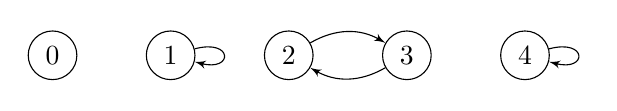
\begin{tikzpicture}
        \tikzset{vertex/.style = {shape=circle,draw,minimum size=1.5em}}
        \tikzset{edge/.style = {->,> = latex'}}
        % vertices
        \node[vertex] (0) at (0,0) {0};
        \node[vertex] (1) at (1.5,0) {1};
        \node[vertex] (2) at (3,0) {2};
        \node[vertex] (3) at (4.5,0) {3};
        \node[vertex] (4) at (6,0) {4};
        %edges
        \draw[edge] (1) to [loop right] ();
        \draw[edge] (2) to [bend left] (3);
        \draw[edge] (3) to [bend left] (2);
        \draw[edge] (4) to [loop right] ();
        
    \end{tikzpicture}

    \caption{Each number points to its inverse modulo 5}
    \end{figure}

    Another thing we can deduce from the fact that $a \times Z_p$ is the same set as 
    $Z_p$ is Fermat's Little Theorem. Ignore $0$ from both the sets and take their product.
    When we equate this, we get: $1 \times 2 \times \dots \times (p-1)
    = a \times 2a \times \dots \times (p-1)a \mod p$. Simplifying, 
    $(a^{p-1}-1)(p-1)! = 0 \mod p$ and since $gcd((p-1)!,p)=1$, $a^{p-1}=1 \mod p$. 

    Fermat's little theorem can also be used to prove EGZ theorem, which we'll see in the next
    lecture.

    \section{Lecture 10}

    We will now do another proof of EGZ theorem for the case where $n$ is prime. It's
    enough to prove this theorem for numbers belonging to $Z_p$, as we only care about 
    remainders when divided by $p$.

    Given a set $S = \{a_1, a_2, \dots, a_{2p-1}\}$, there exists a subset $A \subseteq S$,
    $|A| = p$ and $sum(A) = 0 \mod p$.

    Assume it is not true, that is for all sets the sum is not 0. Let's look at the following sum: \\
    $\sum_{A \subseteq S, |A|=p} (sum(A))^{p-1} \quad (1)$. This is just adding the sum power $p-1$ for all 
    subsets of size $p$. If none of the sums are 0, we can use FLT to show $(sum(A))^{p-1} = 1 \mod p$.
    So the weird sum we're looking at just becomes a summation of $1$, which just counts the number
    of subsets. This is clearly $\binom{2p-1}{p}$. Is this divisible by $p$? \\
    $\binom{2p-1}{p} = \frac{(2p-1)(2p-2)\dots(p)}{(p)(p-1)\dots(1)}$. The $p$'s cancel,
    and nothing else in the numerator is divisible by $p$, so no.

    We'll now show that actually the sum is $0$, by showing that each term in (1) expanded
    is $0 \mod p$. What are possible terms in the summation? For set $A = \{a_{i_1}, a_{i_2},
    \dots, a_{i_p}\}$. We multinomially expand $(a_{i_1} + \dots + a_{i_p})^{p-1}$. A general
    term of this expansion is $a_{i_1}^{k_1}a_{i_2}^{k_2} \dots a_{i_m}^{k_m}$ (call this term $t$) where 
    $1 \leq m \leq p-1$ as you can have maximum $p-1$ different $a_i$'s in a term. We also have 
    $k_1 + \dots k_m = p-1$. Note that $t$ appears multiple times in set $A$ itself, so each 
    set will have a contribution of $k \times t$. What we now prove is that the \emph{number}
    of sets $A$ for which term $t$ appears is divisible by $p$ (which makes its contribution in 
    the final sum as $0 \mod p$).
    \footnote{
    Note that if the term appears in different sets, it will appear the same number of times in 
    each set.
    }
 
    The number of sets in which the term $t$ appears is equivalent to the number of sets that 
    can be formed using the elements $a_{i_1}, a_{i_2}, \dots, a_{i_m}$. Since we have $m$
    elements already chosen and we need to choose $p$ in total, number of elements to be chosen 
    is $\binom{2p-1-m}{p-m}$. \\
    $\binom{2p-1-m}{p-m} = \frac{(2p-1-m)(2p-2-m)\dots(p)}{(p-m)(p-m-1)\dots(1)}$. Since
    there's a $p$ in the numerator, and none of the terms in the denominator are divisible
    by $p$, so the full term is divisible by $p$. 

    So we're done, we got a contradiction. We got that $(1)$ is both $0$ and not $0$ at the 
    same time.

    $2p-1$ is also a tight bound. We have proved the statement for $2p-1$ numbers, but for 
    $2p-2$ numbers we can actually get a counterexamples. Consider the set with $0$ appearing
    $p-1$ times and $1$ appearing $n-1$ times. Any $p$ numbers we choose, we'll have to choose
    2 numbers that differ. If this is the case, the sum is strictly between $0$ and $p$, which 
    means that the sum is not divisible by $p$.

    The theorem can be extended to 2 dimensions. If you have a set of $4p-3$ 2D integer coordinates,
    You can find $p$ of them with their centroid (basically mean of both coordinates) as an
    integer. This theorem was proven and again there's a counterexample with $4p-4$ points. Take 
    the set: \\
    $\{ \binom{0}{0}, \dots, \binom{0}{0}, \binom{0}{1}, \dots, \binom{0}{1}, 
    \binom{1}{0}, \dots, \binom{1}{0}, \binom{1}{1}, \dots , \binom{1}{1}\}$ where each point
    appears $p-1$ times. You will have to choose 2 unequal points, and in whichever coordinate they
    are unequal, that coordinate's sum will be strictly between $0$ and $p$.

    Another theorem we can prove for primes is \textbf{Wilson's Theorem: }a number $n$
    is prime $\iff$ $(n-1)!+1 = 0 \mod n$. 

    The proof of Wilson's Theorem follows from the fact that every number in $Z_p$ (except 0)
    has a unique inverse. So while multiplying all of them, we can just pair each element with 
    its inverse and it will become multiplication of a bunch of $1$'s. But we have to be a bit 
    careful, as what if a number is the inverse of itself? If $a^2 = 1 \mod p$, $(a+1)(a-1)
    = 0 \mod p$. $p \mid (a-1)$ or $p \mid (a+1)$ which means $a = 1$ or $a = p-1$. So ignoring
    these 2 numbers, if we multiply the rest, the product is $1 \mod p$. Including $1$ and $p-1$ now,
    the product is $(p-1) \mod p$, so $(p-1)! + 1 = (p-1) + 1 = 0 \mod p$. 
    
    \newpage
    The converse isn't too hard to prove. 
    One number in $(p-1)!$ will be a divisor of $p$ (say $k > 1$), which will make $(p-1)!$
    also divisible by $k$. Even while taking this modulo $p$, the remainder will be divisible by $k$ as
    if $(p-1)! = qp + r$, $k \mid (p-1)!$, $k \mid p$, so $k \mid r$. From here we can say $r \neq p-1$
    as if $k \mid r = p-1$ and $k \mid p$, $k \mid p - (p-1) = 1$.

    Wilson's theorem is true both ways and can be used as a test for primes, although not efficient.
    The same can't be said for FLT, it is possible when there's a composite $n$, $gcd(a,n)=1$,
    and $a^{n-1} = 1 \mod n$. In fact there are numbers called Carmichael numbers (pseudo primes).
    These are the strongest counterexamples, they are composite $n$ such that for \emph{all}
    $a$ such that $gcd(a,n)=1$, $a^{n-1}=1 \mod n$. The first 3 Carmichael numbers are 561, 1105, and 
    1729.

    There is a way to improve FLT to test more accurately for primes, called the Miller
    Rabin primality test. It's based on FLT as well as the fact that if  $x^2 = 1 \mod n$,
    $x = 1 \mod n $ or $x = n-1 \mod n$. To test if $n$ is prime, we pick a random number
    $1 < a < n$. If $a^{n-1} \neq 1 \mod n$, we confirm $n$ is composite. But if it's equal,
    we're still not guaranteed that $n$ is prime. What we do is we divide the exponent by $2$
    whenever possible, and check if it's still $\pm 1 \mod n$. So we check $a^{\frac{n-1}{2}} \mod n$.
    If it's not $\pm 1 \mod n$, $n$ is composite. If it's $1 \mod n$ and the exponent is still
    even, we can continue this process and check for $a^{\frac{n-1}{4}} \mod n$. If it's 
    $-1 \mod n$, or the exponent becomes odd, we stop, as we can't apply the property anymore.

    Even this test doesn't guarantee if $n$ is prime or composite, but it's better than just 
    plain FLT, as we are checking more. If we do this process for more and more $a$'s, our guarantee
    that $n$ is prime becomes more and more certain. If we ever get that $n$ is composite 
    from the test, we are 100\% sure that it is composite. But if can't disprove $n$ is prime, 
    we are never completely sure that $n$ is prime.

    \section{Lecture 11}

    This lecture is basically discussion of 2 questions in the previous year's quiz.

    \begin{exercise}
        Find natural numbers $n$, $0 \leq n < 1000$ such that $n^2$ has the same ending 3 digits 
        as $n$. Let's generalize this question. What are the number of solutions $0 \leq n < b^d$ 
        such that $n^2$ has the same $d$ ending digits as $n$? It's given that $b$ has a prime 
        factorization $p_1^{k_1}p_2^{k_2} \dots p_m^{k_m}$
    \end{exercise}

    \begin{solution}
        Here's a proof for the general case, just substitute $b = 10$ and $d = 3$ for 
        the first part. When we say the $d$ ending digits are same, we just mean that 
        $b^d \mid (n^2-n)$ or $b^d \mid n(n-1)$. Since $b^d = p_1^{dk_1}p_2^{dk_2} \dots p_m^{dk_m}$,
        it is enough to verify that $p_i^{dk_i} \mid n(n-1)$ for all $i$.
        \footnote{This follows from the fact that if $gcd(d_1,d_2) = 1$, $d_1 \mid n$ and 
        $d_2 \mid n$ $\iff$ $d_1d_2 \mid n$. This can be proved using Exercise 7.1}

        Now since $gcd(n,n-1)=1$, $p_i^{dk_i} \mid n(n-1)$ is equivalent to $ p_i^{dk_i} \mid n$
        or $p_i^{dk_i} \mid (n-1)$. This is like an exclusive or also, we can't have both at the 
        same time. So for every $i$ we have a choice, we could make the term divide $n$ or 
        divide $n-1$. So there are $2^m$ total choices.

        Now for each choice, do we always have a solution, and how many solutions do we have?
        For the extreme cases, when everything has to divide $n$, $n=0$ is the solution. When
        everything has to divide $n-1$, $n=1$ is the solution, but we can't keep checking every
        case manually. Let's say we choose some $d_1$ of these terms to divide $n$ and the rest
        $d_2$ terms to divide $n-1$. Denote the product of the $d_1$ terms to be $t_1$, product
        of the $d_2$ terms to be $t_2$. We have $t_1t_2 = b^d$.

        Since $t_1 \mid n$, we can write $n = qt_1$. To keep $n$ in our range, $0 \leq q < t_2$.
        We need $t_2 \mid n-1 = qt_1-1$ which is basically $qt_1 = 1 \mod t_2$. This is the same
        as saying $q$ is the inverse of $t_1 \mod t_2$. And since $gcd(t_1, t_2) = 1$, $q$ exists
        and is unique. So for each choice we have exactly $1$ solution, so our final answer is $2^m$.
        
    \end{solution}

    \begin{exercise}
        If $\alpha, \beta$ are irrational and $1/\alpha + 1/\beta = 1$, show that for every integer 
        $n$, there exists $k$ such that $n = \floor{k\alpha}$ or $n = \floor{k\beta}$.
        If $\alpha, \beta$ are rational a general solution can be written as $\alpha = \frac{p}{q}$
        and $\beta = \frac{p}{p-q}$ ($gcd(p,q)=1$). For which $n$ (if any) is the statment false? 
    \end{exercise}

    \begin{solution}
        One of the fractions $1/\alpha$, $1/\beta$ must be greater than half. WLOG take it
        to be the first one i.e. $\alpha < 2$. Because it's smaller than $2$, if we think about
        the set $\{\floor{\alpha}, \floor{2\alpha}, \floor{3\alpha}, \dots\}$, it can only skip
        1 number in a row. If it skips a particular $n$, we try to show that there is a $k$ 
        such that $\floor{k\beta} = n$.

        When it skips a particular $n$, say $\floor{k\alpha} = n-1$ and 
        $\floor{(k+1)\alpha} = n+1$
        So the first equation can be written like $n-1 < k\alpha < n$. Note that there's no equality
        as $\alpha$ is irrational. Let's try to manipulate this to be in terms of $\beta$. \\
        $\frac{k}{n-1} > \frac{1}{\alpha} > \frac{k}{n}$ \\
        $\frac{k}{n-1} > 1 - \frac{1}{\beta} > \frac{k}{n}$ \\
        Simplifying, we get $(n-k)\beta > n$ and $(n-k-1)\beta < n-1$. \\
        We can do this for the other inequality too (or just sub $n=n+2$ and $k=k+1$), we get: \\
        $(n-k)\beta < n+1$ and $(n-k+1)\beta < n+2$. \\
        Now from these inequalities, we get $\floor{(n-k)\beta} = n$ so we have found $k' = n-k$
        for which $\floor{k'\beta} = n$.

        In the case of rationals, the only change in our proof is equality in a few inequalities.
        The changes are $n-1 \leq k\alpha < n$ and $ n+1 \leq \floor{(k+1)\alpha} < n+2$.
        This changes the inequality in the last step to $(n-k)\beta \leq n+1$. So our proof
        fails for rationals whenever equality occurs. Tracing this back, it is when $(k+1)\alpha = n+1$.
        i.e. $n = (k+1)\frac{p}{q} - 1$. Since $n$ is natural and $gcd(p,q)=1$, $\frac{k+1}{q}$
        must be an integer, say $k'$. So $n = k' - 1$. Our proof for rationals fails 
        whenever $n = -1 \mod p$.

    \end{solution}

    \section{Lecture 12}

    \textbf{Euler's $\phi$ function: }$\phi(n)$ is the number of no.s $m$ such that
    $1 \leq m \leq n$ and $gcd(m,n) = 1$ or in other words, the number of numbers $m$ smaller than
    $n$ and relatively prime to $n$. This set of numbers is commonly denoted by $Z_n^*$, just
    like how numbers modulo $n$ are denoted with $Z_n$. $Z_n^*$ is just a subset of these numbers
    which are coprime with $n$.

    $Z_n^*$ is also the set of numbers which have a multiplicative inverse modulo $n$. To see why this
    is true, we first show that if $gcd(n,k) = d > 1$, $k$ doesn't have a multiplicative inverse. If $k$
    had a multiplicative inverse $k'$, $kk' = 1 \mod n$, which is same as saying $kk' = qn + 1$.
    But $d \mid kk'$, and $d \mid qn$, so $d \mid 1$, which is a contradiction. To show that any element 
    $a$ in $Z_n^*$ has a multiplicative inverse, we just consider the set $a \times Z_n$ and observe that all
    elements are distinct. If $n \mid a(i-j)$, $n \mid (i-j)$ as $gcd(a,n)=1$, so $i=j$. You can also
    think of $\phi(n)$ as $|Z_n^*|$ (number of elements in the set).

    Let's try to work out $\phi(n)$ for different $n$. When $p$ is prime, $\phi(p)=p-1$ as all numbers
    smaller than $p$ are coprime with it. We can also work out $\phi(p^k)$. If $n$ is a power of 
    a prime, the only numbers which can possibly share a common factor ($>1$) with $n$ are 
    multiples of $p$. So $\phi(p^k) = p^k - p^{k-1} = p^k(1-\frac{1}{p})$, subtracting all multiples of $p$. For other 
    cases it's a bit more complicated. 

    A useful property of $\phi$ is that it's multiplicative. If $gcd(m,n)=1$ then $\phi(mn)
    = \phi(m)\phi(n)$. This actually follows from the \emph{Chinese Remainder Theorem}, so let's 
    prove that first.

    \textbf{Chinese remainder theorem: }If $gcd(m,n)=1$ then for any $a \in Z_m$ and $b \in Z_n$
    there is a unique $c \in Z_{mn}$ such that $c = a \mod m$ and $c = b \mod n$.

    \emph{Proof: }First we show the existence of such a $c$. $gcd(m,n)=1$ means that 
    there are $x,y$ such that $xm + yn =1$. Now we cleverly consider $c = xbm + yan$.
    \begin{flalign*}
        c &= xbm + yan \mod m&&\\
        &= yan \mod m&&\\
        &= (1-xm)a \mod m&&\\
        &= a \mod m&&
    \end{flalign*}
    Similarly, 
    \begin{flalign*}
        c &= xbm + yan \mod n&&\\
        &= xbm \mod n&&\\
        &= (1-yn)b \mod n&&\\
        &= b \mod n&&
    \end{flalign*}

    Now we need to prove that such a $c$ is unique, suppose there are $c_1$ and $c_2$
    which satisfy the conditions. This would mean $c_1-c_2 = 0 \mod m$ and $c_1-c_2 = 0
    \mod n$. Since $gcd(m,n) = 1$, we can say $c_1-c_2 = 0 \mod mn$ so $c_1 = c_2$ (in $Z_{mn}$ 
    at least).

    We can use this theorem to prove $|Z_{mn}^*|=|Z_m^*||Z_n^*|$. From the above theorem,
    we know that for every $a \in Z_m^*$ and $b \in Z_n^*$ we have a unique $c$ in $Z_{mn}$.
    (Since if a number is in $Z_m^*$ it's obviously in $Z_m$, and then we can use CRT). Is 
    $c$ also in $Z_{mn}^*$? If $c$ shared a common factor with $mn$, there would be a common prime
    factor of $c$ and either $m$ or $n$, cause $gcd(m,n) = 1$. WLOG say $d \mid m$ and $d \mid c$.
    But since $c = a \mod m$, $c = qm + a$, so $d$ will also divide $a$. But if $d \mid m$ and 
    $d \mid a$, $d$ has to be $1$ as $a,m$ are coprime. Similarly we can prove that if $d$ is a 
    common divisor of $n$ and $c$, $d = 1$ is forced. So either way we can say $c \in Z_{mn}^*$.

    So each pair of numbers in $Z_m^*$ and $Z_n^*$ corresponds to a unique number in $Z_{mn}^*$.
    So equating the number of cases on both sides, we get $|Z_{mn}^*|=|Z_m^*||Z_n^*|$ i.e.
    $\phi(mn) = \phi(m)\phi(n)$.

    This property helps in deriving a general formula for $\phi(n)$ with its prime factorization.
    If $n = p_1^{k_1}p_2^{k_2} \dots p_m^{k_m}$,
    \begin{flalign*}
        \phi(n) &= \phi(p_1^{k_1})\phi(p_2^{k_2}) \dots \phi(p_m^{k_m})&&\\
        &= p_1^{k_1}(1-\frac{1}{p_1})p_2^{k_2}(1-\frac{1}{p_2}) \dots p_m^{k_m}(1-\frac{1}{p_m})&&\\
        &= n(1-\frac{1}{p_1})(1-\frac{1}{p_2})\dots(1-\frac{1}{p_m})&&
    \end{flalign*}

    There are many ways to derive this formula for $\phi(n)$. Another way is using the principle
    of inclusion exclusion. We want to subtract all numbers which share a $gcd$ greater than $1$
    with $n$. So we subtract multiples of $p_1, p_2, \dots p_m$ from $n$. For each $p_i$, there are
    $\frac{n}{p_i}$ multiples of $p_i$ which are $\leq n$. But if we do this, we are overcounting.
    Some are multiples of $p_i$ and $p_j$, so they are subtracted twice, so we need to add them
    back. But again if we re-add all these cases we'll again face an issue with multiples of 3 
    or more primes, so we continue this process until we deal with all cases.

    In the end, we get:
    \begin{flalign*}
        \phi(n) \quad = \quad &n&&\\
         - &\frac{n}{p_1} - \frac{n}{p_2} \dots -\frac{n}{p_m}&&\\
         + &\frac{n}{p_1p_2} + \frac{n}{p_1p_3} \dots + \frac{n}{p_{m-1}p_m}&&\\
           &\vdots&&\\
         + &(-1)^m \frac{n}{p_1p_2 \dots p_m}
    \end{flalign*}

    This huge mess is just the expansion of $n(1-\frac{1}{p_1})(1-\frac{1}{p_2})\dots(1-\frac{1}{p_m})$.

    There's a similar way to think about this formula, which is more of an intuition rather than a 
    proof, but still might be useful. Again the idea is to delete all the multiples of $p_1, p_2, 
    \dots p_m$.
    Out of all the numbers from $1$ to $n$ a fraction $\frac{1}{p_1}$ of them are multiples of $p_1$, so 
    we remove them and have $n(1-\frac{1}{p_1})$ remaining numbers. Out of these again a fraction
    $\frac{1}{p_2}$ of them will be divisible by $p_2$. Here it's less obvious why it's exactly 
    that fraction (as we don't have a set of consecutive numbers)
    , but here's the intuition. All we have done is removed multiples of $p_1$, and 
    in no way does that tell you anything about if it's a multiple of $p_2$, i.e. divisibility by 
    $p_1$ and $p_2$ are like independent events. So again we multiply by $1 - \frac{1}{p_2}$ to 
    remove the multiples and we continue this idea. In the end, we directly get the formula.

    \begin{exercise}
        It turns out that CRT can be generalized. Let $n_1, n_2, \dots n_k$ be pairwise
        coprime numbers. There's a unique number $c$ in $Z_n$ such that $c = a_i \mod n_i$
        for all $i$. ($a_i$'s are some fixed numbers) How would you find such a $c$ given
        $a_i$'s and $n_i$'s. (Here $n = n_1n_2 \dots n_k$)
    \end{exercise}

    \begin{solution}
        We can just induct on $k$. Given $n_1, n_2$ we know $c = xa_2n_1 + ya_1n_2$
        will satisfy the first 2 modular conditions. 
        Also $c \mod n_1n_2$ is fixed from the uniqueness of CRT. 
        Now that we know what $c$ is modulo $n_1n_2$ and modulo 
        $n_3$, we can find $c \mod n_1n_2n_3$ (as $n_1n_2$ and $n_3$ are also coprime). 
        We can keep continuing this process to find 
        a $c$ which satisfies everything.

        Another method: let's try find a solution of the form 
        \[c = x_1 \frac{n}{n_1} + x_2 \frac{n}{n_2} + \dots x_k \frac{n}{n_k}\]
        We try to toggle the $x_i$'s such that our condition holds. Note that $\frac{n}{n_i}$
        is just the product of all $n_j$'s where $j \neq i$.
        So how does this help, how do we ensure $c = a_i \mod n_i$. In this representation,
        all $\frac{n}{n_j}$'s are divisible by $n_i$, where $j \neq i$. So every term modulo 
        $n_i$ is 0, except for the term $x_i\frac{n}{n_i}$. This is the benefit of our representation,
        $c \mod n_i$ is only affected by $x_i$. Since $n_i$ and $\frac{n}{n_i}$ are coprime, we 
        will have a unique $x_i$ such that $x_i\frac{n}{n_i} = a_i \mod n_i$. We just do this for all
        $i$ and that fixes $c \mod n_i$ for each and every $i$.
    \end{solution}

    \newpage
    \section{Lecture 13}

    Here's another property of $\phi(n)$: $\sum_{d \mid n} \phi(d) = n$. This is saying,
    for every divisor $d$ of $n$, if you sum $\phi(d)$, the result is $n$. We can prove 
    this combinatorially. The RHS is just number of elements in the set $\{1,2,\dots,n\}$.
    For the RHS if we can somehow partition this set into groups where each group has size
    equal to each term in our summation, we are done.

    Partition the set based on the gcd of each number with $n$. For example one group will
    be $Z_n^*$, where each number has gcd $1$ with $n$. All groups will have gcd as some
    divisor of $n$, and all these groups are non-empty, as $d$ (the divisor itself) should
    be in its own group. But how many elements are in each group? So if $gcd(a,n)=d$, 
    we can write $a = da', n = dn'$. gcd of $a',n'$ must be $1$ as if not, $a,n$ would
    have a common divisor bigger than $d$. This is a necessary and sufficient condition
    to ensure $gcd(a,n)=d$. So we just need to count the number of $a'$ coprime with $n' = \frac{n}{d}$
    This is just $\phi(\frac{n}{d})$. So adding the number of elements in each set, we get 
    $\sum_{d \mid n} \phi(\frac{n}{d}) = n$. But we can just rewrite this summation to get 
    our result. If $d$ is a divisor of $n$, clearly $\frac{n}{d}$ is also a divisor. So intead 
    of summing over $d$, we could sum over $\frac{n}{d}$, and we get our result.

    There's another way to show this using the same idea. Look at all the fractions \\
    $ \{\frac{1}{n}, \frac{2}{n}, \dots, \frac{n-1}{n}, \frac{n}{n} \} $ \\ 
    after each fraction is reduced to the simplest form. Once reduced, all fractions would
    have a denominator as some factor of $n$. For each denominator $d$, how many fractions are
    there? Clearly the numerator must be coprime with $d$ so there can be atmost $\phi(d)$
    fractions. We can also say all these fractions will appear, as we can just multiply 
    numerator and denominator to make the denominator $n$, and that fraction reduced
    gives our desired fraction. So if we partition our set based
    on the denominator of the most simplified fraction, we prove that $\sum_{d \mid n} \phi(d) = n$.

    We now look at Euler's Theorem which is a generalization of FLT. For any $a \in Z_n^*$
    (that is $gcd(a,n)=1$), $a^{\phi(n)} = 1 \mod n$.

    The proof comes from ideas we've seen before. We consider the set $a \times Z_n^*$.
    Every element of this set is different as if $n \mid a(i-j)$, $n \mid (i-j)$ as $gcd(a,n)=1$
    which would imply $i=j$. Since every element of this set is different, and also every 
    element is in $Z_n^*$, the set is just a permutation of $Z_n^*$ itself. Equatiing the 
    products of each set, we get that \\
    $a_1a_2 \dots a_{\phi(n)} = (aa_1)(aa_2)\dots(aa_{\phi(n)}) \mod n$ \\
    $(a^{\phi(n)} - 1)(a_1a_2 \dots a_{\phi(n)}) = 0 \mod n$ \\
    Since $a_i$'s are all coprime with $n$, we get $a^{\phi(n)} - 1 = 0 \mod n$ i.e.
    $a^{\phi(n)} = 1 \mod n$.

    \textbf{RSA Public Key Cryptography}

    Number theory is widely used in cryptography. A common way of encrypting messages which 
    is still used today is known as RSA Public Key Cryptography. The challenge of cryptography
    is that we need a message to be able to be decoded very easily if and only if you have a 
    key (secret data). But anyone should be able to encode a message and send it to you easily.
    As encoding is the inverse operation of decoding, we need to find some operation which is 
    is easy to do but the inverse is very hard to do, unless you have extra information.

    A common idea is factorization. This is something we still don't know how to do efficiently,
    but obviously we know how to multiply numbers easily. First we choose 2 large primes, $p$ and 
    $q$, and multiply them to get $n = pq$. Clearly $\phi(n) = (p-1)(q-1)$. We then choose $e$
    which is used to encode messages. An important criteria for $e$ that we want is $gcd(e, \phi(n)) 
    = 1$. So this is how our information is shared:
    \begin{itemize}
        \item Public Key: $e$, $n$
        \item Private Key: $p$, $q$
    \end{itemize}
    The public key is information which is shared to everyone, so that anyone can encode and message
    to you. The private key is information which only you should have, used to decode the message.
    So how does encoding work? If you want to encode a message $m$, we send $m^e \mod n$ instead.
    How do we decode the message? We first find the multplicative inverse $d$ of $e \mod \phi(n)$.
    We then raise the encoded message to the power of $d$. This works because of the following:

    $(m^e)^d \mod n$ \\
    $= m^{ed} \mod n$ \\
    $= m^{k\phi(n)+1} \mod n$ (as $ed = 1 \mod \phi(n)$) \\
    $= (m^{\phi(n)})^k \times m \mod n$ \\
    $= m \mod n$ (as $m^{\phi(n)} = 1 \mod n$)

    So we got back our original message. We can see why we needed $gcd(e, \phi(n)) = 1$ we required
    $e$ to have a multiplicative inverse. There's another small thing, in order to use Euler's 
    theorem, we require $gcd(m,n)=1$. But how do we ensure this for all $m$, we want the sender to
    send whatever they want right\dots So what we do is we make sure our message is small, smaller
    than both $p$ and $q$ to be exact. This forces $m$ not to be a multiple of $p$ or $q$, so 
    $gcd(m,n) = 1$ is ensured. If a bigger message is to be sent, break it into chunks and send 
    each chunk separately.

    Now we just have to be sure that this is easy to decode with the private key and hard without it.
    Firstly, encoding is easy, as $m^e$ can be done very quickly. Note that this takes $O(log(e))$ time
    and not $O(e)$ time, doing exponentiation efficiently (without this our algorithm is no good).
    Now for decoding. We first have to find $d$. For this we can use Euclid's algorithm to find
    $x,y$ such that $ex + \phi(n)y = gcd(e, \phi(n)) = 1$. $x$ is actually our required $d$, as 
    from this equation $ex = 1 \mod \phi(n)$. Euclid's algorithm is also logarithmic time, so this is 
    fast. We then raise our encoded message to the power $d$, again fast. Now how can one decode this 
    message without the private key? They would need to find $d$, for which they would need to find 
    $\phi(n)$ first. But $\phi(n)$ can only be found if you know $p$ and $q$. This is technically
    crackable, as $n$ is public knowledge, but computationally not feasible at all. So the algorithm
    is a successful one.

    We move to a new concept called \emph{primitive root}. We know number $a \in Z_p^*$
    satisfies $a^{p-1} = 1 \mod p$ by FLT. Here $p$ is prime so $Z_p^*$ is just $\{1, 2, 
    \dots, p-1\}$. $a$ is called a primitive root if the exponent $p-1$ is the smallest $k$
    such that $a^{k} = 1 \mod p$. Take the example $p = 7$. See the powers of $2$, $2^0 = 1,
    2^1 = 2, 2^2 = 4, 2^3 = 8 = 1$, so $2$ isn't a primitive root. But $3$ is a primitive root 
    modulo $7$ (can be checked manually).

    If $a$ is a primtive root, the set $\{a,a^2, a^3, \dots, a^{p-1}\}$ is just a permutation 
    of $Z_p^*$. If 2 elements were the same, $a^i = a^j \mod p$, so $a^j(a^{i-j} - 1) = 0 \mod p$.
    $a^j$ isn't divisible by $p$ so we get $a^{i-j} = 1 \mod p$. But this contradicts the fact that
    $p-1$ is the smallest number, $i-j$ is a smaller exponent.

    \begin{exercise}
        If $k$ is the smallest (non zero) number such that $a^k = 1 \mod p$, prove that $k \mid p-1$.
    \end{exercise}

    \begin{solution}
        If $k \nmid p-1$, say the remainder when $p-1$ is divided by $k$ is $r$. So 
        $p-1 = qk + r$. So $a^{p-1} = a^{qk+r} = {(a^k)}^q \times a^r$. Taking modulo $p$
        on both sides, we get $a^r = 1 \mod p$ which contradicts the fact that $k$ is the 
        smallest exponent. 

        This argument can be generalized. Note that the only thing we have used in this theorem 
        about $p$ being prime is that $a^{p-1} = 1 \mod p$. If $p$ was not prime, we could have just
        replaced $p-1$ with $\phi(p)$ and our argument still holds. In fact, we can further replace
        $\phi(p)$ with any $x$ such that $a^x = 1 \mod p$. We get a pretty strong result here, any solution
        to $a^x = 1 \mod p$ will be a multiple of $k$.


    \end{solution}

    \begin{exercise}
        From the previous exercise we got that the smallest $d$ such that $a^d = 1 \mod p$
        is a divisor of $p-1$. But how many such $a$ are there for this $d$ such that $d$ is 
        actually the smallest exponent?
    \end{exercise}

    \begin{solution}
        There could be $0$ such $a$, but let's try to find the maximum number of solutions
        for $a$. If there's one $a$, we know that $a, a^2, a^3, \dots, a^d$ form distinct
        a set of numbers in $Z_p^*$. All these numbers satisfy $x^d = 1 \mod p$, as ${(a^i)}^d
        = {(a^d)}^i = 1 \mod p$. These are all the solutions too, as the equation can have at
        most $d$ solutions. But out of these, we need to check how many have $d$ as the smallest
        exponent.

        Take a general term in this set $a^i$, suppose gcd of $d, i$ is  $g > 1$. In that case, we
        can find a smaller exponent, $\frac{d}{g}$. Because ${(a^i)}^{\frac{d}{g}} = 
        {(a^{\frac{i}{g}})}^d = 1 \mod p$. If suppose $i$ is coprime with $d$, then it turns out 
        that $a^i$ is a primitive root. If ${(a^i)}^x = 1 \mod p$, from the generalization of the 
        previous exercise, we get that $ix$ should be a multiple of $d$. But since $i,d$ are coprime
        $x$ should be a multiple of $d$ so $x = d$ is the smallest solution.

        So we get the following result, there are either 0 solutions, or if there is a solution for 
        $d$, there are $\phi(d)$ solutions as that's the number of $i$'s which are coprime with $d$.
    \end{solution}

    We can prove that every prime $p$ will have a primitive root. Let's partition the set
    $Z_p^*$ based on the smallest exponent $d$ such that $a^d = 1 \mod p$. We have proved that 
    all possible $d$ will be divisors of $p-1$, and also for each $d$, there are either $0$
    or $\phi(d)$ solutions. For each $d$ let $S(d)$ be the number of solutions. We know
    $\sum_{d \mid p-1} S(d) = p-1$, as this is just a partition of $Z_p^*$. But $S(d) \leq \phi(d)$
    as $S(d)$ is either $0$ or $\phi(d)$. So we can say 
    \[ p-1 = \sum_{d \mid p-1} S(d) \leq \sum_{d \mid p-1} \phi(d) = p-1 \]

    But since we have equality, we must have $S(d) = \phi(d)$ for all divisors $d$ of 
    $p-1$. And since $S(d) = S(p-1)$ represent how many numbers have smallest exponent
    as $p-1$, we can say there are $\phi(p-1)$ primitive roots. 

    \section{Lecture 14}

    Tutorial with questions on $\phi(n)$

    \begin{exercise}
        Find all natural numbers $n$ such that $\phi(n) \mid n$
    \end{exercise}

    \begin{solution}
        We can solve this using the formula for $\phi(n)$
        We need $\frac{n}{\phi(n)}$ to be an integer. This simplifies to 
        \[ \frac{1}{\prod_{p_i \mid n} (1-\frac{1}{p_i})} = \prod_{p_i \mid n} \frac{p_i}{p_i-1}\]
        where $p_i$'s are distinct primes that divide $n$. WLOG assume $p_i$'s are in
        ascending order.
        If $p_1 \neq 2$, each product term in the numerator is odd and the denominator is even,
        that's not possible. So we must have $p_1 = 2$. This gives us one infinite family of solutions
        $n = 2^k, k \geq 0$ ($k = 0$ includes $n=1$ as a solution). What about $p_2, p_3, \dots$? 
        Even when $p_1 = 2$, the power of $2$ is the numerator is just $1$ so we can have only 1 extra 
        odd prime, else the denominator won't be divided fully. So $p_2$ can exist but no other prime.
        So we want $\frac{2}{1}\frac{p_2}{p_2-1}$ to be an integer. We know $\frac{2p_2}{p_2-1} > 2$
        so the integer it should simplify to must be $\geq 3$. Simplifying $\frac{2p_2}{p_2-1} \geq 3$, 
        we get $p_2 \leq 3$ so $p_2 = 3$ is forced. This gives another set of solutions, $n = 2^a3^b,
        a \geq 1, b \geq 1$.
    \end{solution}

    \begin{exercise}
        Prove that if $m \mid n$, $\phi(m) \mid \phi(n)$
    \end{exercise}

    \begin{solution}
        This follows from the fact that the $\phi$ function is multiplicative.
        If $m \mid n$, every prime power that appears in the prime factorisation
        of $m$ appears in the factorisation of $n$, and the power is higher.
        That is, if ${p_i}^{a_i}$ appears in $m$, we can say ${p_i}^{b_i}$ will appear
        in $n$, where $b_i \geq a_i$.
        So $\phi(m) = \phi({p_1}^{a_1})\phi({p_2}^{a_2})\dots\phi({p_k}^{a_k})$, and
        $\phi(n) = \phi({p_1}^{b_1})\phi({p_2}^{b_2})\dots\phi({p_k}^{b_k})\phi(n')$.

        From here we can see that $\phi(m) \mid \phi(n)$, because corresponding terms divide
        each other. $\phi({p_i}^{b_i}) = {p_i}^{b_i}(1-\frac{1}{p_i})$, and $\phi({p_i}^{a_i}) 
        = {p_i}^{a_i}(1-\frac{1}{p_i})$, so $\phi({p_i}^{b_i}) = p^{b_i-a_i}\phi({p_i}^{a_i})$.
        Since each term divides the other, the product will also divide the other product.

        This fact can also be proved combinatorially when $m$ and $\frac{n}{m}$ are coprime,
        forming a bijection between $Z_n^*$ and $Z_m^* \times Z_{n/m}^*$ using CRT, 
        as done before. But no idea how do do it when they aren't coprime.
    \end{solution}

    \section{Lecture 15}

    We move to a new topic, sets relations and functions. Informally a set is just a collection 
    of objects. We would like our sets to have some concrete mathematical properties, so
    let's try to build them as we go.

    A first property could be that given any element, it should be either in the set, or not in 
    the set. Mathematically, we can say $\forall S \ \forall x, x \in S$ should be a proposition, 
    either true or false. It would seem like this is the only restriction/condition we need on sets,
    but this isn't the case.

    Consider the set $S$ which contains all the objects/sets which don't contain itself. That is
    $S = \{x | x \notin x\}$. We now look at the proposition $S \in S$, is it true or false?
    Suppose it is true i.e $S \in \textbf{S}$. This would mean $S$, being in $\textbf{S}$, satisfies
    the property $S \notin S$. But this is a contradiction. Suppose it is false, $S \notin S$.
    But since $\textbf{S}$ has all objects which satisfy $x \notin x$, $S$ must be in $\textbf{S}$,
    which is again a contradiction.

    How do we resolve this paradox? We need to add more restrictions on how we build sets, we can't 
    just define sets in this way. There are rigorous axioms of set theory which forbid things like 
    what we did above. But for this course, we will make it simpler. We shall assume there are some
    `base' sets which are given to exist, like the natural numbers. And given any set, we are allowed
    to construct subsets. What does this mean? Say $S$ is well-defined. We are allowed to construct
    set $X = \{x | x \in S \land P(x)\}$, where $P$ is some predicate which decides if elements are in $X$
    or not. In the above paradox, while defining $S$, we didn't say from which set we are picking $x$
    from, so it's not allowed.

    Given these conditions, can we say there's a universal set $U$. That is, is there a set $U$ such 
    that $x \in U$ is always true? Because of the same paradox, we can prove that it's not possible.
    Suppose there is such a $U$. We now construct $S = \{x| x \in U \land x \notin x \}$. Look at 
    the proposition $S \in S$. If $S \in \textbf{S}$, we know $S$ should satisfy the property of the 
    set which is $S \notin S$ which is a contradiction. What if $S \notin S$? We can also 
    say $S \in U$ as $U$ is universal, but that would mean $S$ would then satisfy the property of
    the elements of set $\textbf{S}$ which would make $S \in \textbf{S}$. So we have the same
    contradiction.

    Where exactly is our contradiction? It is the fact that we assumed that a universal set $U$ 
    exists. We could argue that maybe we're not allowed to write statements like $S = 
    \{x| x \in U \land x \notin x \}$. But that's a property we \emph{want}, we would like to allow
    constructing subsets from any given set, so we allow it to be true, and conclude that the 
    contradiction is at assuming such a $U$ exists.

    This type of proof is also seen in something known as the \emph{Halting problem}.
    The question is as follows: does there exists a program $H$ which tells if any other
    program terminates for an input? 

    Assume there exists $H$ such that $H(P, input) = yes$, if $P(input)$ terminates and otherwise,
    $H(P, input) = no$.
    Now let's define a new program $H'$. This takes just $P$ as an input. It works
    as follows: it first runs $H(P, P)$\footnote{The second argument to $H$ can also
    be a program as you can convert programs to integers if you want}, 
    if the output is $yes$, $H'$ runs forever. If the output is $no$, the program terminates.

    Now what's the output of $\textbf{H'}(H')$? Let's go step by step, so in order for 
    $\textbf{H'}$ to run $H'$ it first runs $H(H',H')$. We don't really know what's the output
    of this, say the output is $yes$. Then the program ($\textbf{H'}(H')$) would decide to run forever. 
    But $H(H',H')$
    giving output $yes$ means that $H'(H')$ halts, by the definition of $H$. So we have a contradiction.
    If the output of $H(H',H')$ is $no$, then the main program ($\textbf{H'}(H')$) 
    decides to halt. But giving output $no$
    means by definition $H'(H')$ runs forever. Again we have a contradiction.

    Even though there's no universal $U$, we can still have a $U$ and talk about only
    sets which are subsets of $U$. There are other sets but we can limit our focus to 
    exclude them.

    Here are a few operations on sets that we've seen before.
    \begin{itemize}
        \item Union $A \cup B = \{x|x \in A \lor x \in B\}$
        \item Intersection $A \cap B = \{x|x \in A \land x \in B\}$
        \item Set Difference $A - B = \{x|x \in A \land x \notin B\}$
        \item Complement $A^c = \{x| x \notin A\}$
        \item Cartesian Product $A \times B = \{(a,b)|a \in A \land b \in B \}$ (We assume $U \times U$ is defined)
        \item Subset $S \subseteq A$ if $\forall x \ x \in S \implies x \in A$ 
        \item Powerset $2^A = \{x|x \subseteq A\}$ (We assume $2^U$ is defined)
    \end{itemize}

    In fact, real numbers are also defined as subsets of rational numbers which the following
    property: $x \in S \land y \leq x \implies y \in S$. That is if there's a number is $S$, all
    numbers smaller that it are in $S$. The real number denoted by this set is basically the supremum
    (smallest upper bound) of this set.

    For example $\sqrt{2}$ can be denoted by the set $S = \{x| x<0 \lor x^2 < 2\}$. This satisfies
    the given property, as if $y \leq x \in S$, either $y < 0$ or we can say
    $y^2 \leq x^2 < 2$, so $y \in S$ in both cases.
    
    \newpage
    \section{Lecture 16}
    
    Now that we've defined set, we can define relations and functions.

    A relation $R$ is just a subset of $A \times B$. That is, it contains elements of 
    the form $(a,b)$ where $a \in A$ and $b \in B$, satisfying some predicate $P(a,b)$.
    If $(a,b) \in R$, we say `$a$ is related to $b$ by $R$', or we could write it as $aRb$
    too. When $R$ is defined from $A$ to $A$ itself, we call $R$ a relation on set $A$.

    \begin{figure}[ht]
    \centering
    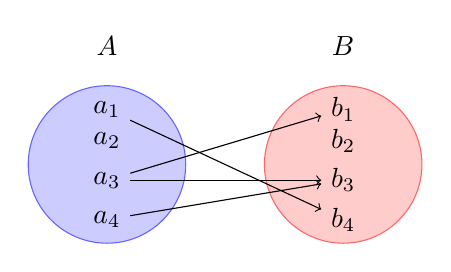
\begin{tikzpicture}
        % draw the sets
        \filldraw[fill=blue!20, draw=blue!60] (-1.5,0) circle (1cm);
        \filldraw[fill=red!20, draw=red!60] (1.5,0) circle (1cm);
    
    
        % the texts
        \node at (-1.5,1.5) {$A$};
        \node at (1.5,1.5) {$B$};
    

        \node (x1) at (-1.5,0.7) {$a_1$};
        \node (x2) at (-1.5,0.3) {$a_2$};
        \node (x3) at (-1.5,-0.2) {$a_3$};
        \node (x4) at (-1.5,-0.7) {$a_4$};
        \node (y1) at (1.5,0.7) {$b_1$};
        \node (y2) at (1.5,0.3) {$b_2$};
        \node (y3) at (1.5,-0.2) {$b_3$};
        \node (y4) at (1.5,-0.7) {$b_4$};
    
        % draw the arrows
        \draw[->] (x1) -- (y4);
        \draw[->] (x3) -- (y3);
        \draw[->] (x3) -- (y1);
        \draw[->] (x4) -- (y3);
    
    \end{tikzpicture}
    \caption{Mapping diagram of relation $R$}
    \end{figure}

    A function is just a special type of relation. It adds the restriction that each element
    $a \in A$ is related to one and only one element $b \in B$ i.e all elements in $A$ have 
    1 image. How do we write this mathematically? We can say that 
    $\forall a \in A \ \exists b \in B \ (a,b) \in R$ which says that every element has at least
    one image. We also add the uniqueness condition now, that's just $(a, b_1) \in R \ \land \ 
    (a, b_2) \in R \implies b_1 = b_2$. So when we write $f(a) = b$, it's just notation for
    $(a,b) \in f$.

    We call a function one-to-one if no 2 elements map to the same number. A function is 
    one-one (injective) when it satisfies $f(a_1) = f(a_2) \implies a_1 = a_2$. A function 
    is onto if all elements of $B$ have an element mapping to it (pre-image). A function is 
    onto (surjective) when it satisfies $\forall b \in B \ \exists a \in A \ f(a) = b$. functions
    which are both one-one and onto are called bijective functions, they are special as there
    is a one-to-one correspondence between both sets. They also have an inverse which is also 
    bijective.

    \begin{exercise}
        If $f$ is a bijective function, define $g$ to be $(b,a) | (a,b) \in f$. Prove that
        $g$ is a function and is bijective.
    \end{exercise}

    \begin{solution}
        We first have to show $g$ is a function. We have to show $\forall a \ \exists b$
        $g(a) = b$, this is identical to showing $\forall a \ \exists b$ $f(b) = a$ which 
        comes from onto-ness of $f$. Then we have to show $g(a) = b_1, g(a) = b_2 \implies 
        b_1 = b_2$ which is equivalent to $f(b_1) = a, f(b_2) = a \implies b_1 = b_2$ which
        comes from one-one-ness of $f$. 

        Now to show $g$ is one-one. $g(a_1) = g(a_2) = b$ (say) $\implies a_1 = a_2$. This 
        is equivalent to $f(b) = a_1, f(b) = a_2 \implies a_1 = a_2$ which is true as $f$ is 
        a function. For showing $g$ is onto we have to show $\forall b \ \exists a \ g(a) = b$
        which is same as $\forall b \ \exists a \ f(b) = a$ which is true as $f$ is a function.
    \end{solution}

    When we want to compare the size of sets, it seems like we can just count the number of elements.
    But this only works when our sets are finite. How we compare 2 sets is by making functions
    from one set to another actually. We can denote $|A| \leq |B|$ if there's a one-one function
    from $A$ to $B$. We can denote $A = B$ if there's a bijection from $A$ to $B$.

    This definition can be a bit counterintuitive for infinite sets, for example it might
    seem like the set of multiples of 3 is smaller than the set of natural numbers, but the 
    function $f(x) = 3x$ is a bijection from $N$ to $3 \times N$. Granted it's correct to say 
    $3 \times N \subset N$ but still we say $|3 \times N| = |N|$.

    We'll now try to prove the theorem $|A| < |2^A|$, which is saying that the power 
    set is strictly smaller than the set itself. To do this we can first show $|A| \leq 
    |2^A|$, as we have the one-one function $f(x) = \{x\}$ (we map $x \in A$ to the singleton
    set $\{x\}$). This is clearly one-one as if $f(x) = f(y) \implies \{x\} = \{y\} \implies
    x = y$.

    Now for the hard part, we still have do disprove equality, by showing there's no
    bijection from $A$ to $2^A$. Assume such a mapping $f$ exists. This maps every element
    $x \in A$ to a set $S \subseteq A$. Now let's look at the set $B = \{x | x \in A \land 
    x \notin f(x)\}$. $B$ is well-defined as it's constructed as a subset of $A$, it could even
    be an empty set but that has nothing to do with whether it's defined. Since $B$ is a subset
    of $A$, $B \in 2^A$, and as $f$ is surjective there is a $b$ such that $f(b) = B$. Now let's 
    consider the proposition $b \in B$. If $b \in B$ is true, $b$ must satisfy the predicate 
    inside $B$, which is $b \notin f(b)$. But $f(b) = B$ which would mean $b \notin B$ which is 
    a contradiction. If $b \in B$ is false. We can say $b \notin f(b)$ as $f(b)$ is same as $B$.
    But then this would mean $b \in B$ as $b$ satisfies the predicate condition of $B$. Either 
    ways, we have a contradiction.

    It turns out that $N$ and $N \times N$. To show this, we need to find a bijection.
    For finding bijection of any set $S$ with naturals, it's enough to find a way to index
    the elements of $S$ with naturals, as our function can be just $f(i) = S[i]$. So we just 
    need to find a way to traverse all the numbers in $N \times N$. If you visualize a $N \times
    N$ as a grid of coordinates, we can traverse all of them by just moving along the diagonals,
    and going to the next one once all elements of a diagonal are covered.

    \begin{figure}[ht]
    \centering
    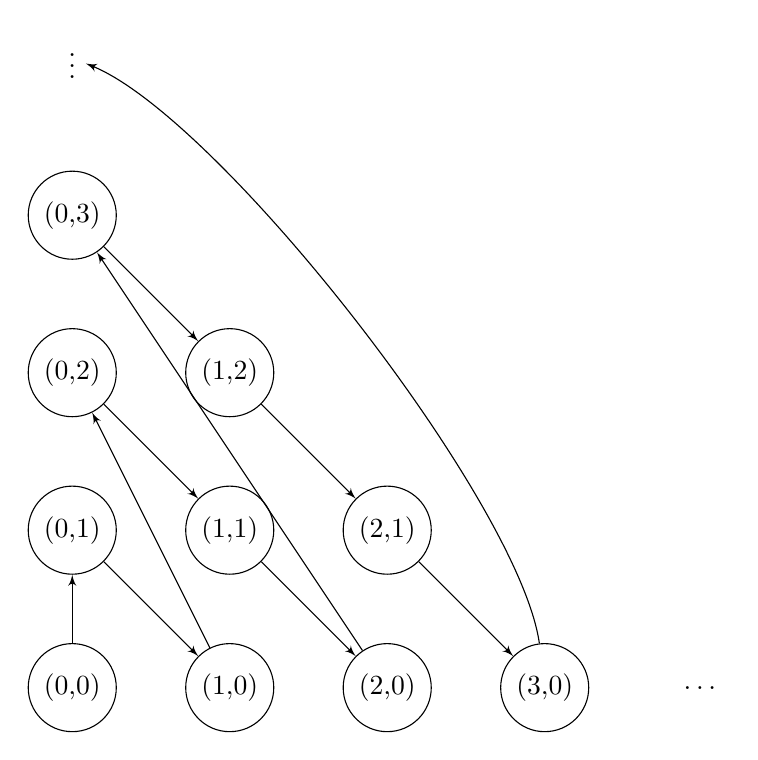
\begin{tikzpicture}
        \tikzset{vertex/.style = {shape=circle,draw,minimum size=1.5em}}
        \tikzset{edge/.style = {->,> = latex'}}

        % vertices
        \foreach \d in {0,1,2,3}
            \foreach \x in {0,...,\d}
                \pgfmathtruncatemacro\y{\d-\x}
                \node[vertex] (\x-\y) at (2*\x,2*\y) {(\x,\y)};

        \node (e1) at (0,8) {\vdots};
        \node (e2) at (8,0) {\ldots};

        %edges
        \foreach \d in {1,2,3}
            \pgfmathtruncatemacro\p{\d-1}
            \foreach \x in {0,...,\p}
                \pgfmathtruncatemacro\t{\x+1}
                \pgfmathtruncatemacro\y{\d-\x}
                \pgfmathtruncatemacro\q{\y-1}
                \draw[edge] (\x-\y) to (\t-\q);

        \foreach \x in {0,1,2}
            \pgfmathtruncatemacro\p{\x+1}
            \draw[edge] (\x-0) to (0-\p);

        \draw[edge] (3-0) to [bend right, looseness=0.5] (e1);

    \end{tikzpicture}
    \captionsetup{justification=centering}  % <-- Center the caption
    \caption{Bijection from $N$ to $N \times N$}
    \end{figure}
    
    It turns out this can be generalized, $|N| = |N^k|$ for any finite $k$. However
    $|N| \neq |N^N|$ where $N^N$ can be thought of the set of all functions from $N$
    to $N$.

    From a theorem we proved, we know that $|N| < |2^N|$. But is there any infinite set
    $S$ is the middle i.e $|N| < |S| < |2^N|$? In words, is there a set $S$ such that there's 
    a non-bijective one-one function from $N$ to $S$ and a non-bijective one-one function
    from $S$ to $2^N$?

    The claim that there's no such $S$ is called the \emph{Continuum Hypothesis}. This 
    stood as an unsolved problem for a long time. It was finally proven that the hypothesis 
    was not true, not false, but unsolvable. That is, it was shown that using the axioms of set
    theory, it is impossible to prove or disprove the Continuum Hypothesis.\footnote{
    How does someone even prove something can't be proven
    }

    So based on if you assume the hypothesis to be true or false, you can get different
    axioms of set theory, which will be consistent in their own constructions, but 
    disagree with each other.

    \section{Lecture 17}

    Quiz paper distribution and solutions :|

    \section{Lecture 18}

    \textbf{Schr\"{o}der-Bernstein Theorem:} For any 2 sets $A$ and $B$, there exists a bijection
    between $A$ and $B$ if and only if there exists a one-one function from $A$ to $B$ and there
    exists a one-one function from $B$ to $A$.

    If there exists a one-one function from $A$ to $B$, we denote it by $|A| \leq |B|$. So this 
    theorem is basically $|A| \leq |B| \land |B| \leq |A| \iff |A| = |B|$.

    One way of proving this theorem is easy, if there's a bijection, that function itself is one-
    one, and its inverse exists and is one-one too. But the other way is much harder.

    Assume we have $g: A \rightarrow B$ and $h: B \rightarrow A$ are both one-one. We have to 
    construct $f$ such that $f$ is bijective. We first look at the image of $h$, define set
    $A_0$ as the set of all the elements of $A$ which are not mapped to by $h$. Or rigorously,
    $A_0 = \{ a \in A | \forall b \in B \ h(b) \neq a \}$. Now after we define $A_0$, we map all
    the elements of it to $B$ using $g$, and all the elements of this set back to $A$ using $h$.
    We now call this set $A_1$. Now in $A_1$, we map everything to $B$ and back to $A$ to get 
    set $A_2$. We continue this process and define $A_i$ inductively. \\
    $A_i = \{a \in A | \exists a' \in A_{i-1} \ h(g(a')) = a \}$ \\
    Now what we do is we take union of all such $A_i$'s, until infinity and make a new set. 
    So $A_\infty = \cup_{i=0}^{\infty} A_i$
    \footnote {If you're confused as to how this is well defined think of the set as 
    $\{a | \exists i \ x \in A_i \}$}.

    
    \begin{figure}[ht]
    \centering
    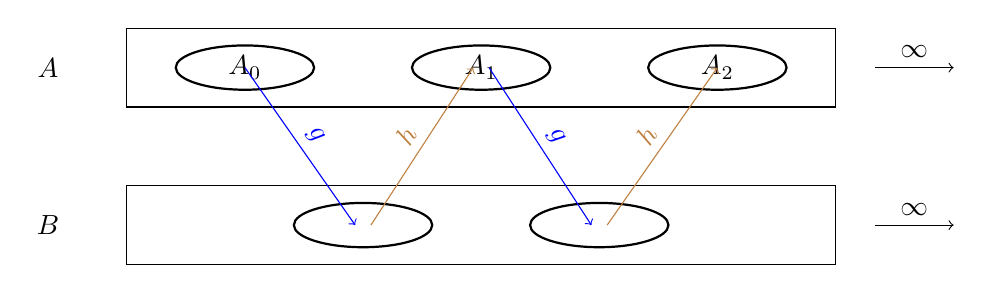
\begin{tikzpicture}
    % Draw the horizontal rectangles
    \draw (0,0) rectangle (9,1);
    \draw (0,-1) rectangle (9,-2);
    
    % Labels for the rectangles
    \node at (-1,+0.5) {$A$};
    \node at (-1,-1.5) {$B$};
    
    % Labels for the top partitions and ellipses
    \node at (1.5,0.5) {$A_0$};
    \node at (4.5,0.5) {$A_1$};
    \node at (7.5,0.5) {$A_2$};
    \draw[thick] (1.5,0.5) ellipse (25pt and 8pt);
    \draw[thick] (4.5,0.5) ellipse (25pt and 8pt);
    \draw[thick] (7.5,0.5) ellipse (25pt and 8pt);
    
    % Label for the bottom partitions and ellipses
    \node at (3,-1.5) {};
    \node at (6,-1.5) {};
    \draw[thick] (3,-1.5) ellipse (25pt and 8pt);
    \draw[thick] (6,-1.5) ellipse (25pt and 8pt);
    
    % Arrows from top ellipses to bottom ellipses with labels
    \draw[->, color=blue] (1.5,0.5) -- (2.9,-1.5) node[midway, above, sloped] {$g$};
    \draw[->, color=brown] (3.1,-1.5) -- (4.4,0.5) node[midway, above, sloped] {$h$};
    \draw[->, color=blue] (4.6,0.5) -- (5.9,-1.5) node[midway, above, sloped] {$g$};
    \draw[->, color=brown] (6.1,-1.5) -- (7.5,0.5) node[midway, above, sloped] {$h$};
    
    % Add an arrow to indicate infinity
    \draw[->] (9.5,0.5) -- (10.5,0.5) node[midway, above] {$\infty$};
    \draw[->] (9.5,-1.5) -- (10.5,-1.5) node[midway, above] {$\infty$};

    \end{tikzpicture}
    \captionsetup{justification=centering}  % <-- Center the caption
    \caption{Diagrammatic explanation as to how $A_i$ is defined}
    \end{figure}

    Now we finally construct our bijection $f$.
    \begin{equation*}
    f(x)=
        \begin{cases}
            g(x) & \text{if } x \in A_\infty\\
            h^{-1}(x) & \text{if } x \notin A_\infty
        \end{cases}
    \end{equation*}

    Now what do we even mean by $h^{-1}$, $h$ is not necessarily a bijective function
    right. But we can still say there's a unique $b \in B$ such that $h(b) = x$ only when
    $x \notin A_\infty$. Why? Firstly, if $x \notin A_\infty$, $x \notin A_0$ as $A_\infty$
    is a superset of $A_0$. But if $x \notin A_0$, we do have a $b$ such that $h(b) = x$ because
    $A_0$ is defined as all elements not in the image of $h$, any element not in it will have an 
    image. And this image is unique, as $h$ is one-one. So even though we don't have bijectivity
    of $h$, $h^{-1}$ is well defined here.

    First let's prove $f$ is one-one, say $f(x_1) = f(x_2)$, we have to prove $x_1 = x_2$. We 
    split by cases. If both $x_1$ and $x_2$ are in $A_\infty$, we have $g(x_1) = g(x_2)$
    so $x_1 = x_2$ as $g$ is one-one. If both aren't in $A_\infty$, we have $h^{-1}(x_1)
    = h^{-1}(x_2)$, applying $h$ on both sides, we get $x_1 = x_2$. Now if they are in different
    sets, say $x_1 \in A\infty$ and $x_2 \notin A\infty$. We have $g(x_1) = h^{-1}(x_2)$,
    $h(g(x_1)) = x_2$. But since $x \in A_i$ for some $i$, $h(g(x_1))$ is in $A_{i+1}$ by how 
    $A_{i+1}$ is constructed. This is a contradiction as we assumed that $x_2 \notin A_\infty$.

    Now to prove onto. For all $b \in B$ we need to prove there's an $a \in A$ such that $f(a) = b$.
    We smartly choose $a = h(b)$. Now if we are lucky enough that $a \notin A_\infty$, 
    $f(a) = h^{-1}(a) = h^{-1}(h(b)) = b$, so $a = h(b)$ works. But what if $a \in A_\infty$?
    $a \in A_i$ for some $i$. We can say for sure $i \neq 0$, as $a = h(b)$ and $h$ doesn't
    map anything to $A_0$. So $i > 0$. We have some $a' \in A_{i-1}$ such that $h(g(a')) = a$
    by construction of $A_i$'s. But as $h$ is one-one and $h(g(a')) = h(b)$, $g(a') = b$. Also 
    since $a' \in A_\infty$, $f(a') = g(a') = b$, so we found a pre-image of $b$ in this case too.

    Since we prove $f$ is one-one and onto, it is a bijection.

    This theorem is very useful when we want to prove that there exists a bijection between 2 sets,
    but it's hard to construct an explicit bijection. For example take the sets $2^N$ and $N^N$. We'll
    prove that they have the same cardinality by creating a one-one function both ways. Here $2^N$ 
    is the set of all subsets of $N$ and $N^N$ is the set of all functions from $N$ to $N$.

    For one-one function from $2^N$ to $N^N$, map each subset of $N$ to the boolean function which decides
    if a number is inside the set. Basically for set $A$, map it to the function $f$ which is like this:

    \begin{equation*}
        f(x)=
            \begin{cases}
                1 & x \in A \\
                0 & x \notin A
            \end{cases}
    \end{equation*}

    Why is this one-one? Given the function $f$ we should be able to get $A$. We just look at where the 
    function is $1$, and only those elements are in our set.

    Now for the other way. We have to map every function to a subset of $N$. So we map $f$ to the following
    set: \\
    $A =\{f(0), f(0)+f(1)+1, f(0)+(1)+f(2)+2, \dots \}$.
    Now we have to show this is one-one, we have to retrieve $f$ from set $A$. The way we have written it,
    the elements of the set are in strictly increasing order. So to retrieve $f(0)$ we find the smallest 
    element in the set. To get $f(1)$, we just see the second smallest element. Since we already know $f(0)$
    we can find $f(1)$. Similarly to find $f(2)$ we look at the third smallest element. Inductively, we 
    can find $f(i)$ for every $i$.

    Now that we have one-one functions both ways, we are guaranteed to have a bijection. Note that neither
    of the one-one functions we found are bijective. The first one only maps to boolean functions, and the
    second one only maps to infinite sets. Finding an explicit bijection will be too hard.

    We now look at a few operations on relations. To really visualize these, we introduce another way
    to see relations. Since $R$ is a subset of $A \times B$, we can mark which elements of $A \times B$
    are in $R$, and which aren't. This is just a boolean matrix of $A \times B$.

    \[
    \begin{array}{c|cccc}
        R & b_1 & b_2 & \ldots & b_n \\
        \hline
        a_1 & 1 & 0 & \ldots & 0 \\
        a_2 & 1 & 0 & \ldots & 1 \\
        \vdots & \vdots & \vdots & \ddots & \vdots \\
        a_m & 1 & 1 & \ldots & 0 \\
    \end{array}
    \]

    In this matrix, we have $a_i R b_j$ if $R[i][j] = 1$ in the matrix, and they're not 
    related if $R[i][j] = 0$. When sets $A$ and $B$ are infinite, our matrix is also infinite.

    So our first operation is \emph{converse}. We define $R^{-1}$ from $B$ to $A$, such that 
    $b R^{-1} a = a R b$. These are just the tuples in $R$ which are swapped. If we want to represent 
    this as a matrix, $R^{-1}$ is just the transpose of $R$.

    Another operation is composition. If we have $R_1: A \rightarrow B$ and $R_2: B \rightarrow
    C$. We define $R_1 \cdot R_2 = \{(a,c) | \exists b \  (a,b) \in R_1 \land (b,c) \in R_2\}$.
    Basically if $aR_1b$ and $bR_2c$, we can say $a \ R_1 \cdot R_2 \ c$. It turns out this is same 
    as boolean matrix multiplication. Let's derive this. If $a_iRc_j$, there should be $k$ such 
    that $a_iRb_k$ and $b_kRc_j$. So we must have $a_iRb_1 \land b_1Rc_j$, or $a_iRb_2 \land b_2Rc_j$,
    or ... This is summation terms, simplifies to $\sum_{r=1}^{k} a_iRb_r \land b_rRc_j$ where we treat 
    summation as logical or. This is exactly how we define matrix multiplication.

    Other operations on relations are union and intersection. Since relations are just sets, these are
    defined just how we define them on sets.
    
    For relations on a set $A$, that is $R:A \rightarrow A$, we have some more definitions.
    \begin{itemize}
        \item Identity Relation: $a_1Ra_2 \iff a_1 = a_2$. This would be represented as an identity matrix.
        \item Symmetric Relation: $a_1Ra_2 \implies a_2Ra_1$. This relations form symmetric matrices, and satisfy $R^{-1} = R$.
        \item Transitive Relation: $\forall a_1,a_2,a_3, \ a_1Ra_2 \land a_2Ra_3 \implies a_1Ra_3$
        \item Anti-symmetric Relation: $a_1Ra_2 \land a_2Ra_1 \implies a_1 = a_2$. This is like the opposite of symmetric, 
        basically 2 distinct numbers are never related both ways.
    \end{itemize}

    \section{Lecture 19}

    Relation $R: A \rightarrow A$ is said to be an equivalence relation if it is symmetric, reflexive
    and transitive. 

    Equivalence relations are special, and they can work as an equality operator too. This is because
    when we say 2 things are `equal', we have some predefined notions of equality. Firstly,
    every element is equal to itself. Also if $a = b$ then $b = a$. And finally if $a = b$,
    $b = c$, $c = a$. Now if we just replace `$=$' with `$R$' we get the definition of an equivalence 
    relation.
    
    In fact given a function $f: A \rightarrow B$, define $R$ like this: \\
    $a_1Ra_2 \iff f(a_1) = f(a_2)$. Any such $R$ is an equivalence relation (it can be proved
    by using the properties of `$=$'). Such an $R$ is called the kernel of $f$, it bascially 
    says 2 elements are identical if $f$ maps them to the same thing.

    The converse also turns out to be true. If $R$ is an equivalence relation on a set $A$, 
    there exists a function $f: A \rightarrow B$ such that $R$ is the kernel of $f$, that is 
    $a_1Ra_2 \iff f(a_1) = f(a_2)$.

    \begin{exercise}
        Can you prove the converse explicitly i.e. can you construct the function $f$ given $R$?
    \end{exercise}
    
    \begin{solution}
        Yes you can, take the function as $f : A \rightarrow 2^A$ to be $f(a) =
        \{x|x \in A \land aRx\}$, or in words, $f(a)$ is the set of all elements related to $a$.
        Now to prove that this $R$ is the kernel of $f$. First let's prove that if 
        $aRb$, then $f(a) = f(b)$.
        
        $f(a)$ and $f(b)$ are sets, so we do what we do normally to show 2 sets are equal.
        Assume $x \in f(a)$ i.e $aRx$. Since $R$ is symmetric, $xRa$, and we already have 
        $aRb$ so $xRb$ as $R$ is transitive. This also implies $bRx$ so $x \in f(b)$. So what
        we've done finally is $x \in f(a) \implies x \in f(b)$ i.e. $f(a) \subseteq f(b)$. 
        Similarly we can show $f(b) \subseteq f(a)$ so $f(a) = f(b)$.
        
        Now for the converse, what we'll do is prove if $aRb$ is false, $f(a) \neq f(b)$.
        This is not too hard, as $b \in f(b)$ as $R$ is reflexive, but $b \notin f(a)$ as 
        $aRb$ is false.
    \end{solution}

    From this exercise, we can further say that the kernel of a function $f$ basically partitions
    the set $A$ into non-empty subsets of elements, such that inside a subset, all elements 
    are related to each other. Define $R(a) = \{x|x \in A \land aRx\}$. For all $a$, this 
    set is non-empty as $a \in R(a)$. But we need to show this is a valid partitioning i.e.
    there can't be overlaps between these sets. Specifically, we have to show for any $a, b$,
    $R(a) = R(b)$ or $R(a)$ and $R(b)$ are disjoint. So suppose they were not disjoint, and 
    have a common element $c$. So $aRc$ and $bRc$. But now using the properties of an equivalence
    relation, we can get $aRb$ and once we got that, we can prove $R(a) = R(b)$ in the same way as 
    the exercise (in the exercise, we weren't given an $f$ so we defined $f(a)$ the same way as we did
    for $R(a)$ here). So we're done, $R$ partitions $A$ into disjoint sets. Now showing every 
    element in a set is related to each other can be done by symmetric and transitive properties, 
    as in each set $R(a)$ all elements are related to $a$. So equivalence classes form a partition of the set $A$, and 2 elements are related if and only 
    if they are in the same equivalence class. 

    Take the example $g(n) = n \mod m$. This partitions $N$ into $m$ equivalence classes, which are 
    $\{0,1,2,\dots,m-1\}$ based on the remainder you get when you divide by $m$. Another 
    example is $f(n) = gcd(n,m)$. The equivalence classes here are all the divisors of $m$, 
    as $gcd(n,m)$ has to be a divisor of $m$.

    In this particular case, are $f$ and $g$ related? Yes, as if we know $g(n)$, we also know 
    $f(n)$. This is from the fact that $gcd(n,m) = gcd(n \mod m, m)$. This means $g(n)$ actually
    groups equivalence classes of $f(n)$ into bigger equivalence classes. We call $g(n)$ a 
    \emph{refinement} of $f(n)$, as looking at things the other way around, $g(n)$ takes equivalence
    classes of $f(n)$ and refines/divides them into more equivalence classes.

    \begin{figure}[H]
    \centering
    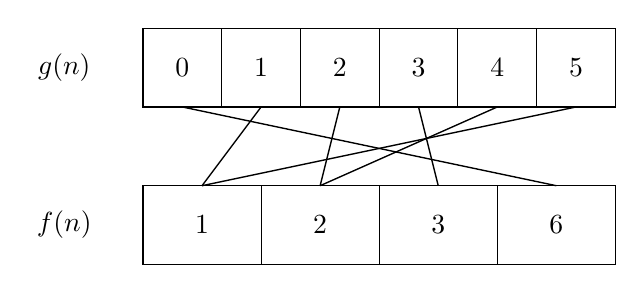
\begin{tikzpicture}
        % Horizontal Rectangle with 6 Boxes
        \draw (0,0) rectangle (6,1);
        \foreach \x in {1,2,3,4,5}{
            \draw (\x,0) -- (\x,1);
        }
        
        % Labeling Boxes
        \foreach \x/\label in {0.5/0, 1.5/1, 2.5/2, 3.5/3, 4.5/4, 5.5/5}{
            \node at (\x,0.5) {\label};
        }
        
        % Vertical Rectangle with 4 Boxes
        \draw (0,-1) rectangle (6, -2);
        \foreach \x in {1.5,3,4.5}{
            \draw (\x,-1) -- (\x,-2);
        }

        % Labeling Boxes
        \foreach \x/\label in {0.75/1, 2.25/2, 3.75/3, 5.25/6}{
            \node at (\x,-1.5) {\label};
        }

        \node at (-1,0.5) {$g(n)$};
        \node at (-1,-1.5) {$f(n)$};

        \draw[line width=0.5pt] (0.5,0) -- (5.25,-1);
        \draw[line width=0.5pt] (1.5,0) -- (0.75,-1);
        \draw[line width=0.5pt] (2.5,0) -- (2.25,-1);
        \draw[line width=0.5pt] (3.5,0) -- (3.75,-1);
        \draw[line width=0.5pt] (4.5,0) -- (2.25,-1);
        \draw[line width=0.5pt] (5.5,0) -- (0.75,-1);

        
    \end{tikzpicture}
    \captionsetup{justification=centering}  % <-- Center the caption
    \caption{Showing how $f(n)$ and $g(n)$ are linked}
    \end{figure}

    Now just like equivalence relations, there's another special type of relation
    called partial order. $R$ is called a partial order on a set $A$ if it is reflexive,
    \emph{anti-}symmetric, and transitive. An example of a partial order we have seen 
    before is just $\leq$. Another partial order which can be defined on a set of sets. 
    $A \ R \ B = $ there is a one-one function from $A$ to $B$ \footnote{For this relation
    we consider 2 sets as equal if their cardinalities are equal, not them being equal
    in the normal sense}. Here what makes this relation anti-symmetric is Schr\"{o}der-Bernstein,
    reflexive and transitive are easier to prove. A subset relation between sets is also
    a partial order i.e. $X_1RX_2$ only when $X_1 \subseteq X_2$.

    \begin{exercise}
        Prove that $R$ is a partial order on a set $A$ if and only if there is an injective function $f: 
        A \rightarrow 2^A$ such that $a_1Ra_2$ if and only if  $f(a_1) \subseteq f(a_2)$
    \end{exercise}

    \begin{solution}
        Let's prove one way first, if the function exists then $R$ is a partial order. $R$ is
        reflexive as $aRa = f(a) \subseteq f(a)$ which is always true. $R$ is also anti symmetric
        as $aRb \land bRa$ is basically $f(a) \subseteq f(b) \land f(b) \subseteq f(a)$. And this 
        means $f(a) = f(b) \implies a = b$ as the function is injective. And for transitive, $aRb \land bRc$
        means $f(a) \subseteq f(b) \land f(b) \subseteq f(c)$. From set properties, $f(a) \subseteq f(c)$
        which means $aRc$.

        Now for the other way, where we are given a partial order $R$ and have to construct a function. We can just
        map each element to the set which it relates to actually. That is, $f(a) = \{x| x \in A \land xRa\}$. Now we 
        have to prove the property $aRb \iff f(a) \subseteq f(b)$. Let's prove it forward first, say $aRb$. Now
        to prove one set is a subset of the other we do our usual method. $x \in f(a) \implies xRa$. But since $aRb$
        and $R$ is transitive, we can say that $xRb \implies x \in f(b)$. So now that we have proved $x \in f(a) \implies
        x \in f(b)$ we conclude $f(a) \subseteq f(b)$. Now say $f(a) \subseteq f(b)$, we have to prove $aRb$. As $R$ is 
        reflexive, $aRa \implies a \in f(a)$. Since $f(a) \subseteq f(b)$, $a \in f(b)$. This means $aRb$, so we are done.
    \end{solution}

    \section{Lecture 20}

    \begin{exercise}
        Suppose there is a bijection from $A \times A$ to $A$. Prove that there exists a bijection from 
        $A \times A \times A$ to $A$. Proceed by induction to show that there's a bijection from $A^k$ to $A$.
 
        We define $A^+ = \cup_{k=1}^{\infty} A^k$ or in words, set of finite sequences of elements from $A$.
        If in addition it's given that $A$ is infinite, then show there's a bijection from $A^+$ to $A$.
    \end{exercise}

    \begin{solution}
        Suppose the bijection we are given is $f$. For the bijection from $A^3$ to $A$, define it 
        as $g_3(a_1, a_2, a_3) = f(f(a_1, a_2), a_3)$. Let's first proof $g_3$ is injective. If $f(f(a_1, a_2), a_3)
        = f(f(b_1, b_2), b_3)$, $f(a_1, a_2) = f(b_1, b_2)$ and $a_3 = b_3$ from the fact that $f$ is injective. And 
        for the same reason, from the first equality we get $a_1 = b_1$ and $a_2 = b_2$. So $g$ is injective. Now for surjectivity,
        we know for all $a$ we can find $x_1, x_2$ such that $f(x_1, x_2) = a$ from the fact that $f$ is surjective. We can 
        also find $y_1, y_2$ such that $f(y_1, y_2) = x_1$. So in the end we have found $y_1, y_2, x_1$ such that
        $f(f(y_1, y_2), x_2) = a$ which is $g_3(y_1, y_2, x_2) = a$ which proves that $g_3$ is surjective.

        
        Induction will work very similarly. For $k=1$, $g_1$ is the identity function, for $k=2$ $g_2 = f$, for 
        $k=3$ we have done above. We define $g_k$ inductively as follows:
        \[ g_k(a_1, a_2, \dots, a_k) = f(g_{k-1}(a_1, a_2, \dots, a_{k-1}), a_k)\footnote
        {I am not going to prove why inductive definitions are valid, but just assume this definition is fine for now, else check Tutorial solutions for rigorous stuff}\]
        \newpage
        Now that $g_k$ is defined, we can prove it is bijective recursively, our base case is the identity function which is easy to prove.
        Suppose $g_k(\bar{a}) = g_k(\bar{b})$ that is $f(g_{k-1}(a_1, a_2, \dots, a_{k-1}), a_k) = f(g_{k-1}(b_1, b_2, \dots, b_{k-1}), b_k)$.
        From the one-one property of $f$, we can say $a_k = b_k$, and $g_{k-1}$ of the rest of the $a_i$'s is equal to $g_{k-1}$ of the rest of the $b_i$'s.
        But from our induction assumption $g_{k-1}$ is one-one, so we get $a_i = b_i$ for all $i$ from $1$ to $k-1$. So this proves
        $\bar{a} = \bar{b}$.

        For surjectivity, we need to find $\bar{x}$ such that $g_k(\bar{x}) = a$ for all $a$. Firstly we can find $x_1, x_2$ such that $f(x_1, x_2) = a$.
        Then from the surjectivity of $g_{k-1}$ we can find $a_1, \dots, a_{k-1}$ such that $g_{k-1}(a_1, \dots, a_{k-1}) = x_1$.
        Now if we just choose $a_k = x_2$ we get $g_k(a_1, \dots, a_k) = f(g_{k-1}(a_1, \dots, a_{k-1}), a_k) = f(x_1, x_2) = a$.
        
        Now for the $A^+$ part of the question. For this part we don't find a bijection explicitly, but find a one-one function both ways. For a one-one function
        from $A$ to $A^+$, we can just have the identity function. Now for the other way.

        Since we're given $A$ is infinite, let us choose an infinite sequence of elements in $A$,
        such that all are distinct, say they are $x_1, x_2, x_3, \dots$\footnote{Again this might seem obviously possible but we need axioms before saying things like this}
        Now for any element in $\bar{a} \in A$, we define our function as follows:
        \[ g(\bar{a}) = f(g_k(\bar{a}), x_k) \text{ where k is the number of elements of } \bar{a} \]
        Now to prove that it is one-one, say $g(\bar{a}) = g(\bar{b})$ which means $g_m(\bar{a}) = g_n(\bar{b})$ 
        and $x_m = x_n$ assuming $\bar{a}$ and $\bar{b}$ have $m$ and $n$ elements respectively. We can conclude $m = n$
        as the set of $x_i$'s are unique. This also means $g_m$ and $g_n$ are the same function, so if $g_m(\bar{a}) = g_n(\bar{b})$
        then $\bar{a} = \bar{b}$ as $g_m$ is bijective hence one-one. So we have proved $g$ is one-one.

        Now that we have a one-one function both ways, there exists a bijection from $A$ to $A^+$

    \end{solution}

    \begin{exercise}
        We have a set $A$ with $n$ elements, and a relation $R$ on $A$. We define a \emph{minimum} element 
        of $A$ as the following. $m \in A$ is minimum if $mRa$ for all $a$, and $aRm \implies a = m$. Suppose that
        $a_iRa_j$ takes some constant time to access, find an algorithm to find the minimum element of $A$ in linear time.
    \end{exercise}

    \begin{solution}
        First of all, not all relations have a minimal element $m$, for example the identity relation. But we can say there can 
        be only 1 minimal element. Say $m_1$ and $m_2$ are minimal elements. $m_1Rm_2$ as $m_1$ is minimum, but from the fact
        that $m_2$ is minimal, $m_1 = m_2$.

        Now for the algorithm, we do something very similar to how we find minimum element of an array. We initialize the minimum
        variable to the first element of the set. Then we iterate through the set, and if $a_iRmin$, weupdate $min$ to be $a_i$. 
        At the end of this loop $min$ will be a candidate for the minimum element. 

        Now why does this algorithm work here too? The idea is the following: no matter what the result of $a_iRa_j$ \footnote{Assuming $i \neq j$}, we can be sure
        one of them is not the minimum element. Suppose $a_iRa_j$ is true, in that case $a_j$ is not the min as $a_iRmin$ is never true when $a_i \neq min$. If 
        $a_iRa_j$ is false, $a_i$ is not the min as $minRa_j$ should always be true. So our algorithm will always have $min$ as a candidate for the minimum. At any 
        stage if we find $a_iRmin$ is false, we continue as we already know $a_i$ is not a candidate. If $a_iRmin$ is true, we know $a_i$ is a candidate so we update 
        the value of $min$ to $a_i$.

        But at the end of this algorithm, we aren't guaranteed the $min$ is actually the minimum of $A$. We need to check for all the elements of $A$ whether $minRa$
        is always true and $aRmin$ is only true when $a = min$. But this also takes linear time, so the algorithm overall is still linear.
    \end{solution}
\end{document}